\documentclass[a4paper,12pt]{article}
\usepackage[utf8]{inputenc}
\usepackage[T1]{fontenc}
\usepackage{amssymb}
\usepackage[polish]{babel}
\usepackage[top=1.5cm, bottom=2.0cm, left=2.5cm, right=2.5cm]{geometry}
\usepackage{indentfirst}
\usepackage{enumerate}
\usepackage{graphicx}
\usepackage[table,xcdraw]{xcolor}




\title{Symulacja natężenia światła}
\author{Paulina Stal, Patrycja Marchwica}
\date{21.05.2020}

\begin{document}
	\maketitle
	
	\section{Wprowadzenie}
	\label{sec:wprowadzenie}
	
	Celem symulacji będzie analiza natężenia oświetlenia w zamodelowanym pomieszczeniu -- sali lekcyjnej. Do przeprowadzenia symulacji zostanie wykorzystany pakiet \emph{VI-Suite}, czyli zintegrowany zestaw narzędzi do analizy otoczenia, wykorzystujący wbudowane funkcje programu do modelowania 3D jakim jest \emph{Blender} oraz integrujący zewnętrzne aplikacje tj. \emph{Radiance}, które umożliwiają przeprowadzenie symulacji oświetlenia.
	
	Pomiar natężenia światła, czyli gęstości strumienia świetlnego padającego na daną powierzchnię, którego jednostką w układzie SI jest luks [lx], zostanie wykonany w różnych miejscach zamodelowanego pomieszczenia. Otrzymane wyniki zostaną poddane analizie, mającej na celu określenie wpływu warunków pogodowych, konfiguracji opraw oświetleniowych oraz mocy świecenia opraw oświetleniowych na przebieg symulacji.  
	

	\section{Potrzebne parametry do opisu modelu}
	 \label{sec:opis_modelu}

	\subsection{Jednostka natężenia}
	\label{subsec:jednostka_natezenia}

	Do scharakteryzowania oświetlenia powierzchni, na którą pada strumien światła przyjmujemy natężenie oświetlenia będącą odpowiednikiem natężenia naprominiowania (irradiancji). Natężenia oświetlenia to nic innego jak gęstość strumienia świtlnego padającego na daną powierzchnię, równa granicy ilorazu strumienia świetlnego $\phi$ padającego na powierzchnię i pola $S$ tej powierzchni, przy $S$ dążącym do zera:
	$$E_{v}=\frac{d \Phi_{v}}{d S}$$
	Jeżeli strumień świetlny pada równomiernie na całą powierzchnie, to:
	$$E_{v}=\frac{\Phi_{v}}{S}$$
Jednostką natężenia oświetlenia w układzie SI jest luks (lx) równy lumenowi na metr kwadratowy $(cd \cdot sr \cdot m^{2})$.
	$$\left[E_{v}\right]=\frac{l m}{m^{2}}=l x$$
	\newpage

	\begin{figure}
  		\centering
    		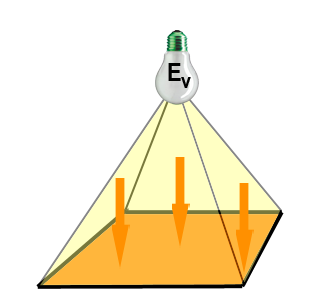
\includegraphics[width=0.5\textwidth]{natezenie_grafika}
		\caption{Graficzne przedstawienie jednostki natężenia oświetlenia.}
	\end{figure}

	\subsection{Stosowane normy natężenia}
	\label{subsec:stosowane_normy}

	Natężenie oświetlenia zostało określone przez normę PN-EN 12464-1:2012. \newline Wymagania oświetleniowe wynikają z uwzględnienia trzech podstawowych potrzeb człowieka:
	\begin{itemize}
		\item wygody widzenia – spostrzeganie jest sprawne, pozbawione ryzyka, nie prowadzi do odczucia niewygody i nadmiernego zmęczenia,
		\item wydolności wzrokowej – zadania wzrokowe można wykonać w trudnych warunkach i w dłuższych okresach czasu,
		\item względów bezpieczeństwa.
	\end{itemize}
	
	Do podstawowych parametrów otoczenia świetlnego wliczających w to światło sztuczne jak i dzienne, zalicza się:
	\begin{itemize}
		\item rozkład luminancji w otoczeniu,
		\item natężenie oświetlenia na polu pracy i w jego otoczeniu,
		\item kierunek światła, oświetlenie w przestrzeni wnętrza,
		\item zmienność światła (poziom i barwa światła),
		\item olśnienie (przeszkadzające, przykre i odbiciowe),
		\item oddawanie barw i barwy postrzeganej
		\item migotanie światła i efekty stroboskopowe.
	\end{itemize}

	Ze względu na wygodę widzenia powinno unikać się we wnętrzach wysokich luminancji, które mogłyby spowodować wzrost olśnienia, czy wysokich kontarstów przyczyniających się do zmęczenie oczu. Niskie luminancje czy niskie kontrasty sprawiają, że środowisko pracy staje się monotonne.
	\newpage
	W normie przyjęto, że wymagane natężenie oświetlenia w celu dostrzeżenia rysów ludzkiej twarzy w normalnych warunkach oświetleniowych, powinno być nie mniejsze niż 20 lx i jest to najmniejsze natężenie oświetlenia wymieniane przez normę. W typowych pracach biurowych, takich jak: pisanie ręczne, pisanie na maszynie, 				czytanie, obsługiwanie klawiatury wymagane jest natężenie oświetlenia 500 lx, dla prac precyzyjnych przewyższa 1000 lx. W słoneczny letni dzień natężenie oświetlenia w miejscach niezacienionych osiąga wartość 100.000 lx.\\

	\noindent Według normy PN-EN 12 464-1: 2004 zalecane natężenie oświetlenia:
	\begin{center}
		\begin{table}[!h]
        		\centering     
			\begin{tabular}{|p{0.6\textwidth}|p{0.1\textwidth}|}
				\hline 
				rozpoznanie rysów twarzy & 20 lx \\
				\hline 
				wykonywanie prostych czynności  & 50 lx \\
				\hline 
				obsługa komputera, prace biurowe & 500 lx \\
				\hline 
				montaż precyzyjny, mikromechanika, zakład jubilerski   & 1000 lx \\
 				\hline
			\end{tabular}     
       		 \end{table}
	\end{center}
	Wartości orientacyjne zależne od różnych czynników, np.: pory roku i dnia, stopnia zachmurzenia czy czystości powietrza):
	\begin{center}
		\begin{table}[!h]
        		\centering     
			\begin{tabular}{|p{0.75\textwidth}|p{0.1\textwidth}|}
				\hline 
				 oświetlenie powierzchni ziemi przez Księżyc w pełni w pogodną noc & 0.2 lx \\
				\hline 
				oświetlenie uliczne w nocy  & 5-10 lx \\
				\hline 
				pomieszczenie od zacienionej strony w środku dnia & 300 lx \\
				\hline 
				oświetlenie słoneczne terenu na zewnątrz (zachmurzone niebo)   & 5000 lx \\
 				\hline
			\end{tabular}     
       		 \end{table}
	\end{center}

	\subsection{Oświetelenie w szkołach}
	\label{subsec:oswietlenie_w_szkolach}

		Oświetlenie sali lekcyjnej powinno zapewniać wygodę widzenia oraz poprawiać zdolność do rozróżniania szczegółów bez nadmiernego zmęczenia wzroku.  Odgrywa istotną rolę w kształceniu uczniów przyczyniając się do efektywnej i przyjemnej pracy. Wymiary standardowej sali lekcyjnej zawierają sie między $55m^{2}$  a 				$62m^{2}$ dla 30 uczniów. Stosunek między powierzchnią okien a podłogą powinien wynosić 1:4 do 1:5. 

		Natężenie oświetlenia w salach lekcyjnych musi wynosić 300 lx natomiast powinno być wysokie (500 lx) tam, gdzie wykonywane są głównie ,,zadania wzrokowe'' -- czytanie i pisanie ręczne. Preferowanym rodzajem źródeł światła do oświetlania pomieszczeń w szkole (klas, korytarzy, szatni) są świetlówki. W warunkach stałego 				rozmieszczenia ławek w klasach zalecane są świetlówki liniowe. Wykorzystywane są różne odmiany świetlówkowych opraw oświetleniowych - wbudowywane w sufit, nasufitowe i do podwieszania pod sufitem.

		Uwzględniając konserwacje przy projektowaniu i instalacji systemów oświetlenia tak aby najdłużej eksploatować oprawy oświetleniowe przy zachowaniu właściwych parametrów światła stosuje się lampy LED.
	\newpage

	\section{Implementacja}
	 \label{sec:implementacja}

	\subsection{Technologie i narzędzia}
	\label{subsec:technologie_i_narzedzia}

		Do zamodelowania sali lekcyjnej jak i do wyrenderowania obrazów został użyty pragram \emph{Blender}. Aby zobrazować natężenie światła w określonych miejsca, zbadać wpływ warunków pogodowych i ustawienia lamp wykorzystano rozszerzenie \emph{VI-Suite}. Analiza oświetlenia została uzyskana poprzez dwa 					komponenty \emph{VI-Suite}: \emph{LiVi}, który spełnia funkcje pre/post-procesora pakietu do analizy oświetlenia - \emph{Radiance} oraz \emph{EnVi}, który zapewnia takie same możliwości dla programu do symulacji poboru energii (między innymi oświetlenia) -  \emph{EnergyPlus}.

	\begin{figure}[!ht]
	\centering
	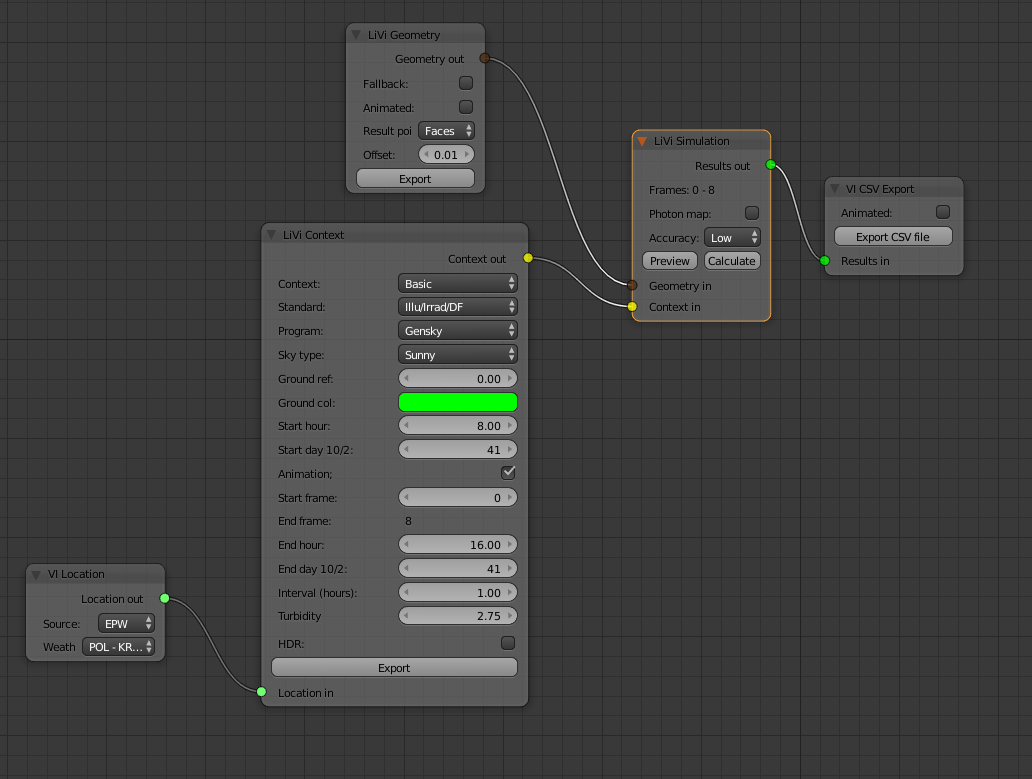
\includegraphics[width=0.8\textwidth]{node_editor}
	\caption{Node Editor}
	\label{node_editor}
	\end{figure}

	\begin{figure}[!ht]
		\centering
		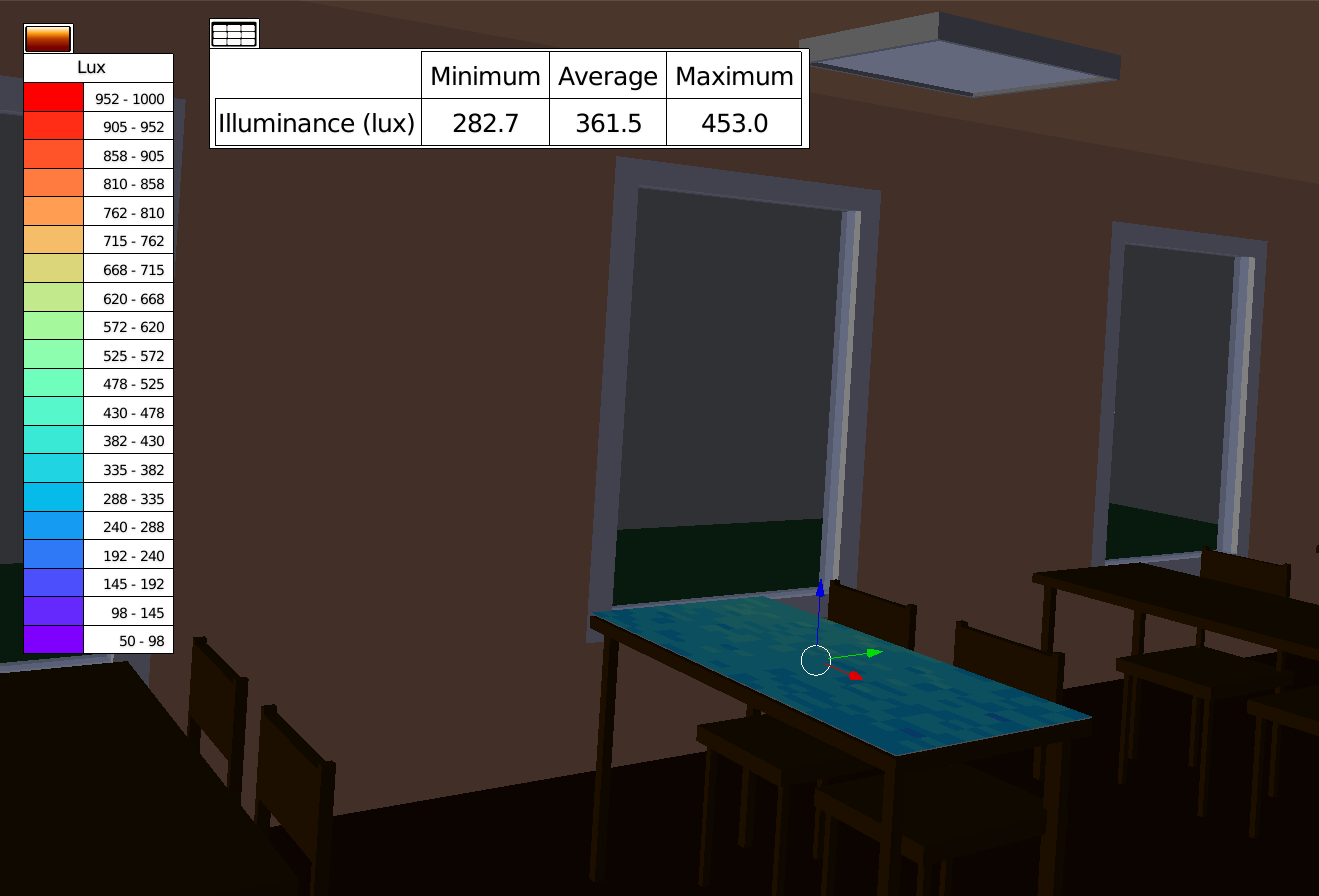
\includegraphics[width=0.8\textwidth]{wynik_symulacji}
		\caption{Wyniki otrzmane w wyniku symulacji}
		\label{wynik_symulacji}
	\end{figure}

	\begin{figure}[!ht]
		\centering
		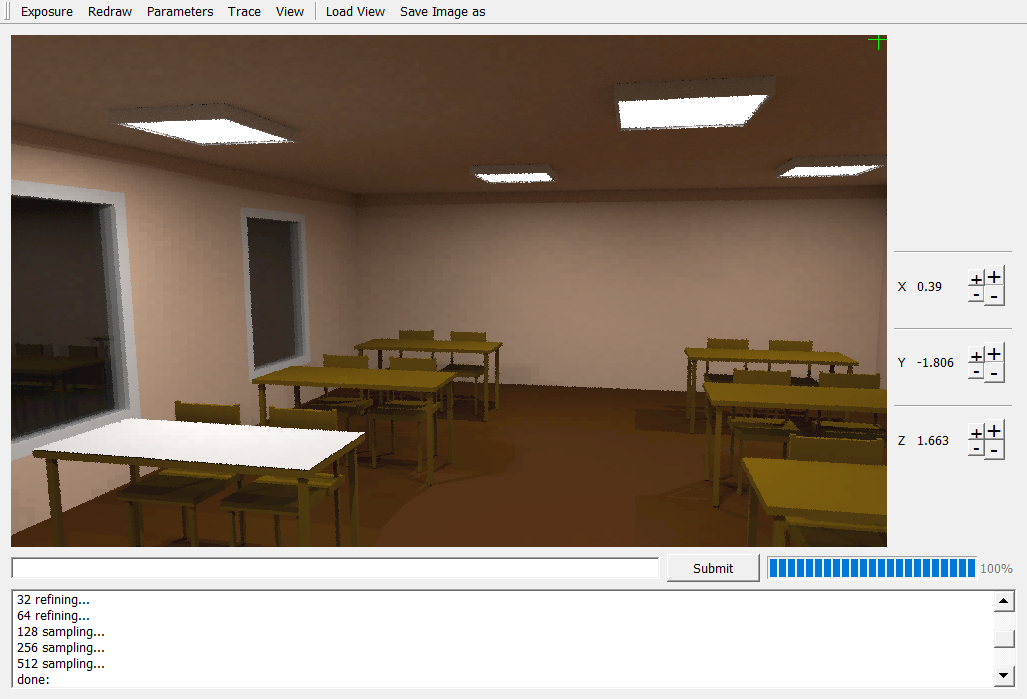
\includegraphics[width=0.8\textwidth]{podglad_symulacji}
		\caption{Podgląd przeprowadzanej symulacji}
		\label{podglad_symulacji}
	\end{figure}



	\subsection{Parametry modelu}
	\label{subsec:parametry_modelu}
	
	\begin{itemize}
		\item Model sali lekcyjnej
		\begin{itemize}
			\item Wymiary modelu sali lekcyjnej -- $6m$ x $10m$ x $2.5m$
			\item Pole powierzchni podłogi -- $60m^2$
			\item Wymiary ławek -- $500mm$ x $1300mm$ x $40mm$
			\item Wysokość ławek ($640mm$) i krzeseł ($38mm$) dostosowana do wzrostu ucznia -- $133-159cm$
		\end{itemize}
		\item Okna
		\begin{itemize}
			\item Stosunek powierzchni okien do powierzchni podłogi -- $1:5$
			\item Wymiary okien -- $1m$ x $1.5m$ x $0.12m$
			\item Odległość pomiędzy oknami -- $1.15m$
			\item Odległość okna od podłogi -- $0.68m$
			\item Okna znajdują się od wschodniej i zachodniej strony pomieszczenia
		\end{itemize}
		\newpage
		\item Oświetlenie
		\begin{itemize}
			\item Typ oświetlenia -- Oświetlenie LED natynkowe
			\item Wymiary opraw oświetleniowych -- $620mm$ x $620mm$ x $66mm$
			\item Temperatura barwowa -- $4000K$
			\item Rozmieszczenie opraw oświetleniowych 1 (Rysunek \ref{konfiguracja_opraw_1}):
			\begin{itemize}
				\item 8 lamp -- w dwóch rzędach po 4 wzdłuż sali lekcyjnej
				\item Odległość pomiędzy oprawami -- $1.13m$
				\item Odległość pomiędzy oprawą a oknami -- $1.48m$
				\item Odległość pomiędzy oprawą a ścianami północną i południową -- $1.43m$
			\end{itemize}
		
		\begin{figure}[h]
			\centering
			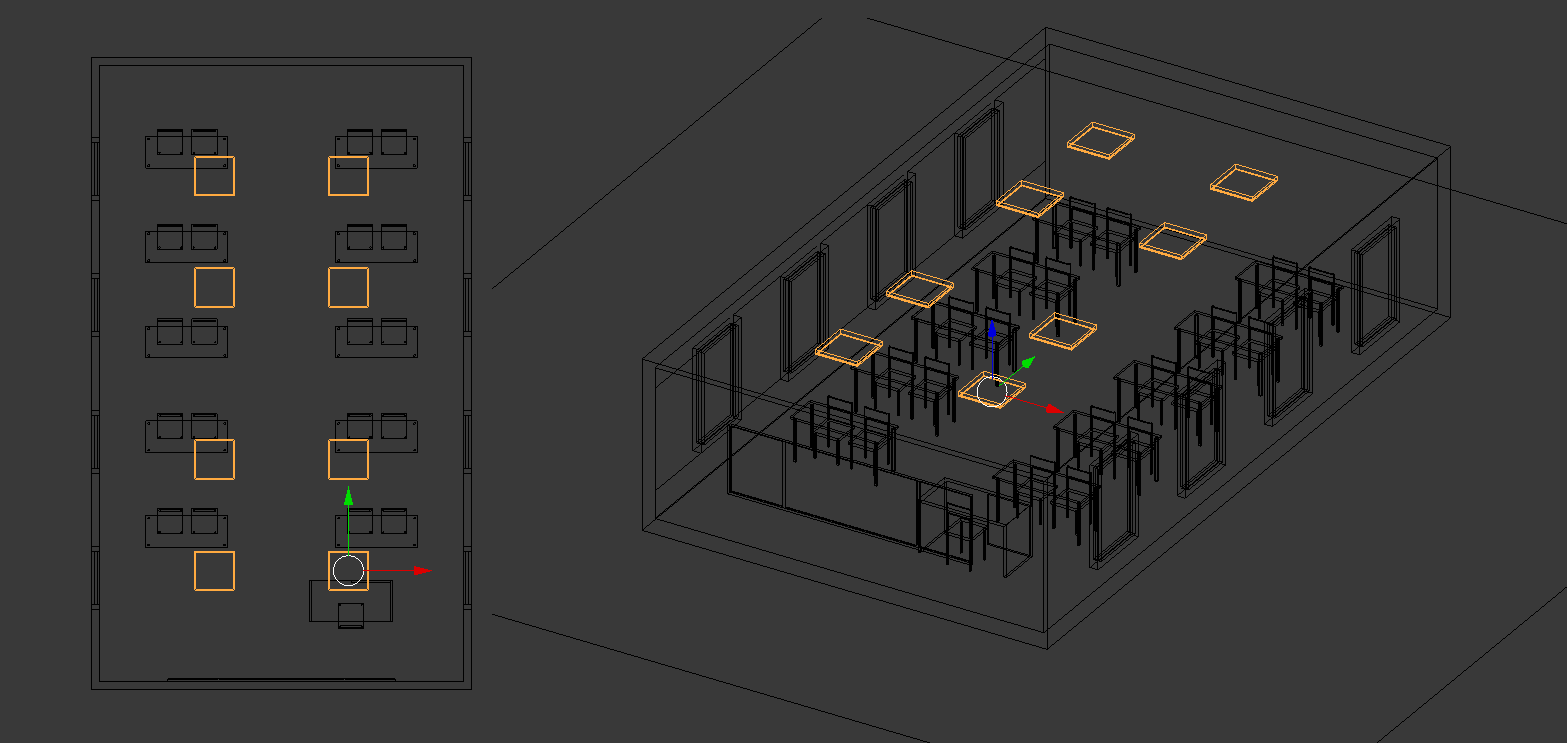
\includegraphics[width=1\textwidth]{konfiguracja_oswietlenia_1}
			\caption{Konfiguracja opraw oświetleniowych nr 1}
			\label{konfiguracja_opraw_1}
		\end{figure}
	
				\item Rozmieszczenie opraw oświetleniowych 2 (Rysunek \ref{konfiguracja_opraw_2}):
			\begin{itemize}
				\item 8 lamp -- w ,,szachownicę''
				\item Odległość pomiędzy oprawami -- $1.80m$
				\item Odległość pomiędzy oprawą a oknami -- $0.75m$ i $1.95m$
				\item Odległość pomiędzy oprawami wzdłuż sali lekcyjnej oraz oprawami a ścianami północną i południową -- $1.45m$
			\end{itemize}	
		\end{itemize}
		\begin{figure}[h]
			\centering
			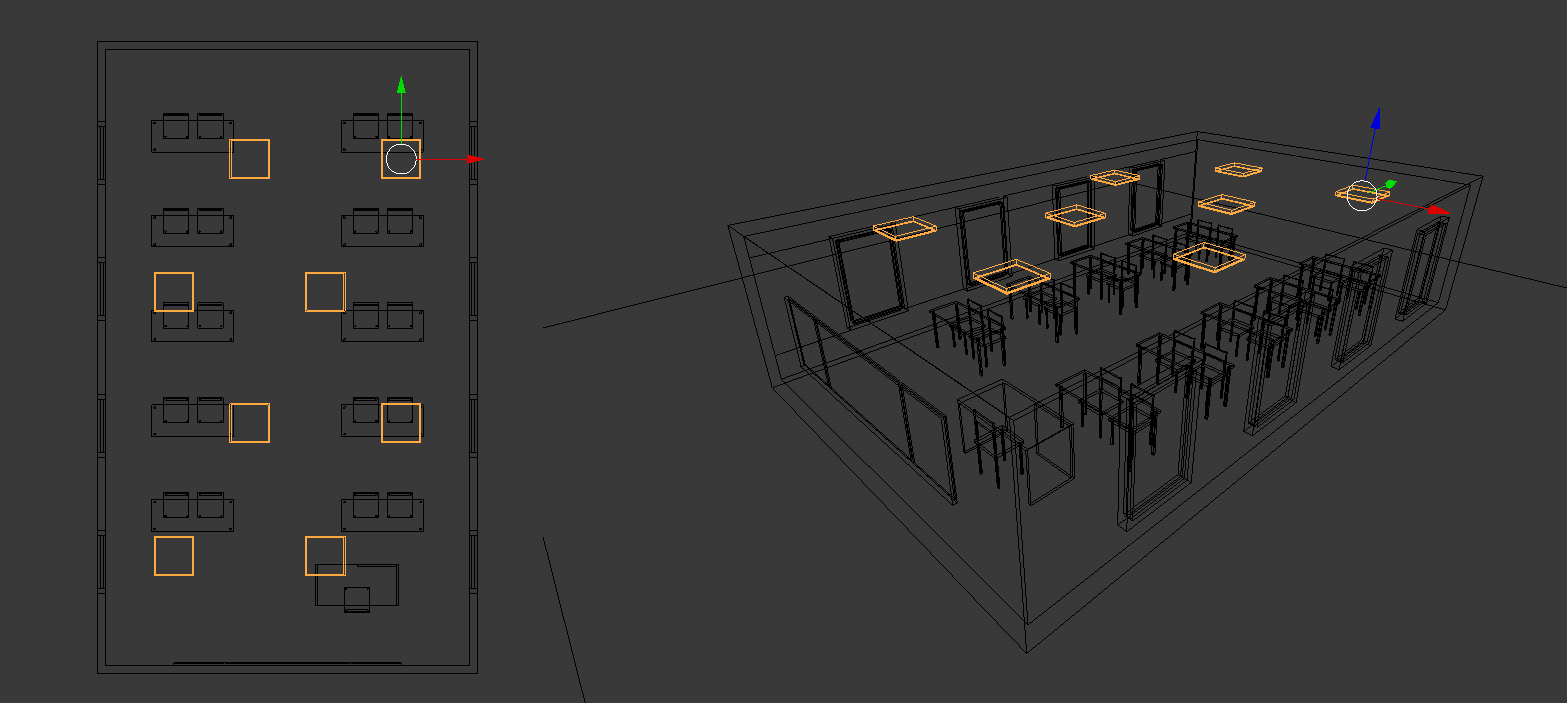
\includegraphics[width=1\textwidth]{konfiguracja_oswietlenia_2}
			\caption{Konfiguracja opraw oświetleniowych nr 2 - ,,szachownica''}
			\label{konfiguracja_opraw_2}
		\end{figure}

		\item Parametry Vi-Suite
		\begin{itemize}
			\item Lokalizacja -- Kraków -- dane zawarte w pliku EnergyPlus weather pobranym z [11]
			\item Pomiar natężenia oświetlenia co 1h pomiędzy 8.00 a 16.00
		\end{itemize}		
		
	\end{itemize}

	\section{Rezultaty}
	\label{sec:rezultaty}
	
	\subsection{Symulacja dla całego roku bez oświetlenia}
	\label{subsec:caly_rok}
	
	\begin{figure}[ht!]
		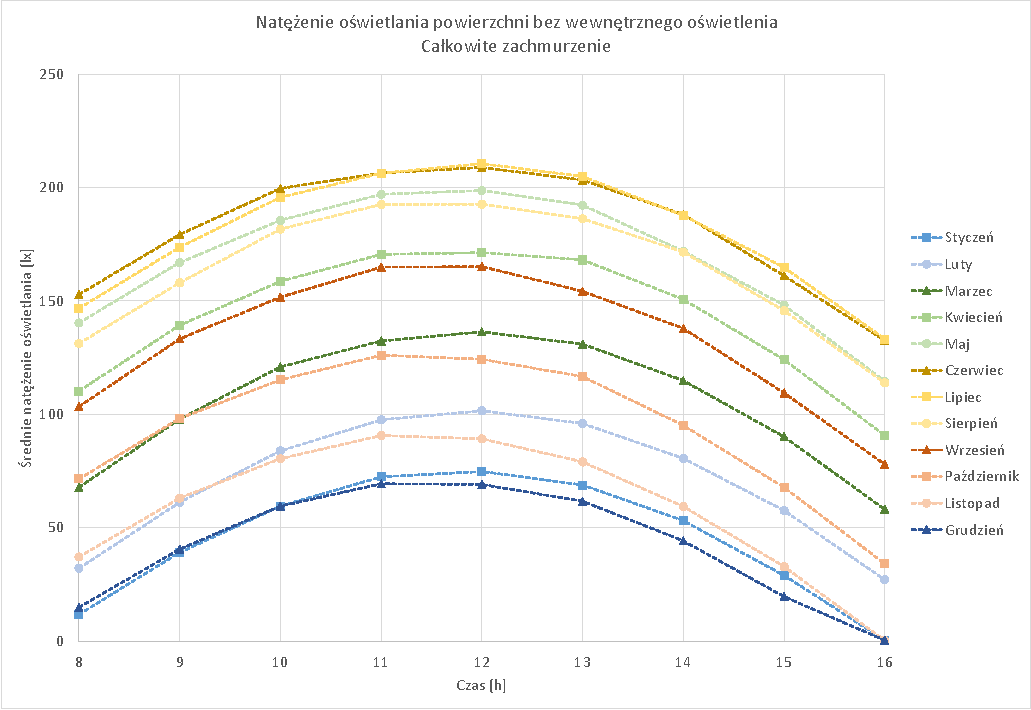
\includegraphics[scale=0.8]{Wykresy/caly_rok.pdf}
		\centering
		\caption{Natężenie oświetlania powierzchni biurka w sali lekcyjnej bez włączonego oświetlenia dla wszystkich miesięcy}
		\label{fig:caly_rok}
	\end{figure}
	
	\subsection{Brak oświetlenia}
	\label{subsec:brak_oswietlenia}
	
	\begin{figure}[ht!]
		\centering
		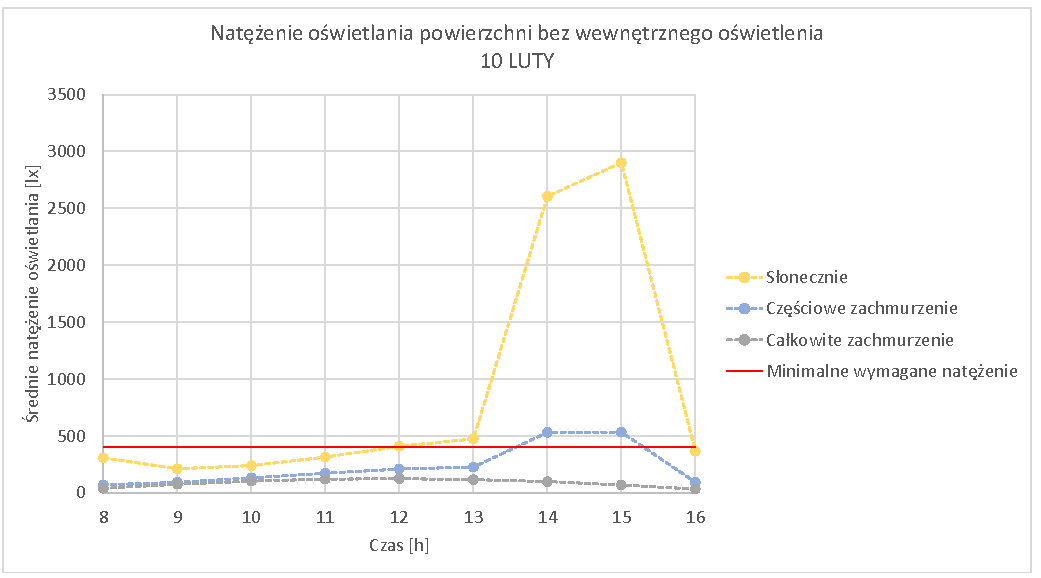
\includegraphics[scale=0.8]{Wykresy/bez_oswietlenia_1.pdf}
		\caption{Natężenie oświetlania powierzchni biurka w sali lekcyjnej bez włączonego oświetlenia dla różnych warunków pogodowych }
		\label{bez_oswietlenia_1}
	\end{figure}

	\subsection{Konfiguracja opraw oświetleniowych 1}
	\label{subsec:oswietlenie_1}

	\begin{figure}[ht!]
		\centering
		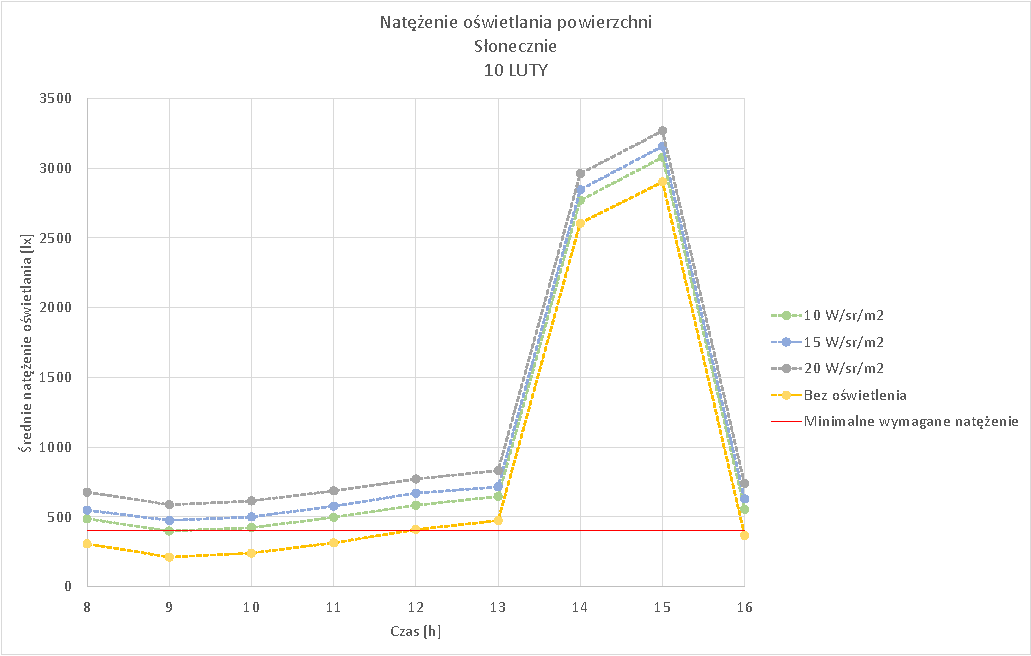
\includegraphics[scale=0.8]{Wykresy/oswietlenie_1_slonecznie.pdf}
		\caption{Natężenie oświetlania powierzchni biurka w sali lekcyjnej w słoneczny dzień przy włączonym oświetleniu dla konfiguracji opraw oświetleniowych nr 1 i różnej wartości radiancji}
		\label{oswietlenie_1_slonecznie}
	\end{figure}

	\begin{figure}[!ht]
		\centering
		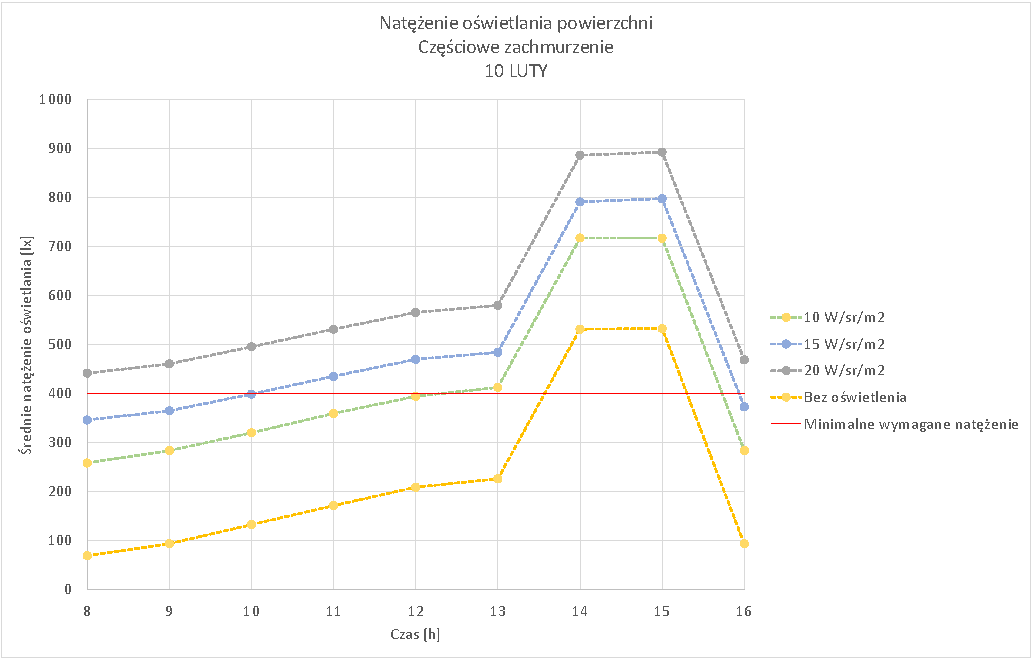
\includegraphics[scale=0.8]{Wykresy/oswietlenie_1_czesciowe_zachmurzenie.pdf}
		\caption{Natężenie oświetlania powierzchni biurka w sali lekcyjnej przy częściowym zachmurzeniu  oraz włączonym oświetleniu dla konfiguracji opraw oświetleniowych nr 1 i różnej wartości radiancji}
		\label{oswietlenie_1_czesciowe_zachmurzenie}
	\end{figure}

	\begin{figure}[!ht]
		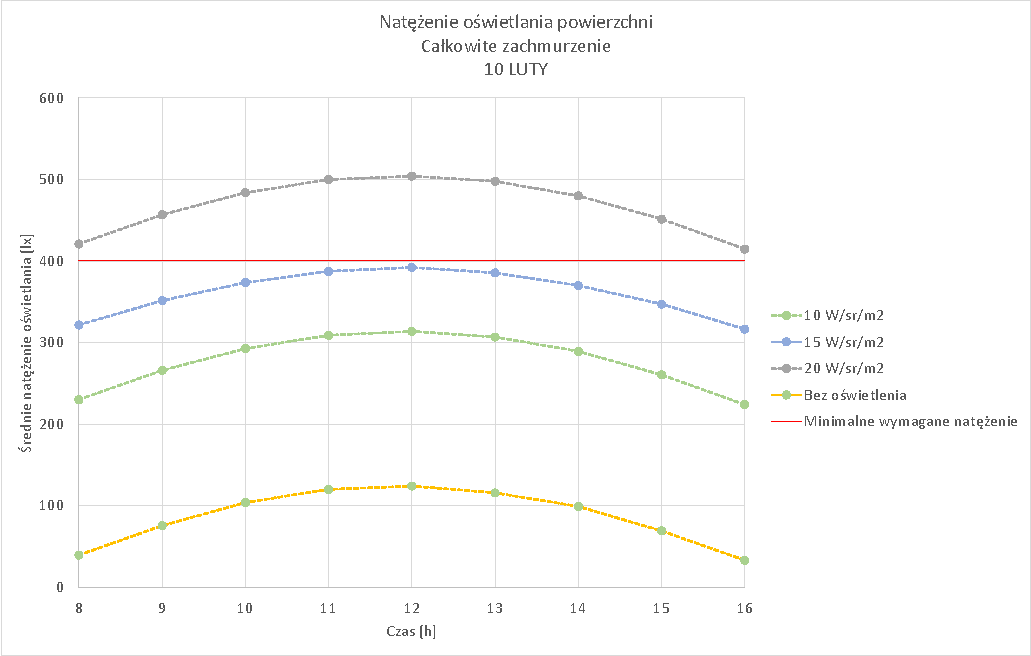
\includegraphics[scale=0.8]{Wykresy/oswietlenie_1_calkowite_zachmurzenie.pdf}
		\caption{Natężenie oświetlania powierzchni biurka w sali lekcyjnej przy całkowitym zachmurzeniu  oraz włączonym oświetleniu dla konfiguracji opraw oświetleniowych nr 1 i różnej wartości radiancji}
		\label{oswietlenie_1_calkowite_zachmurzenie}
	\end{figure}
	\newpage

	\subsection{Konfiguracja opraw oświetleniowych 2}
	\label{subsec:oswietlenie_2}
	
	\begin{figure}[!ht]
		\centering
		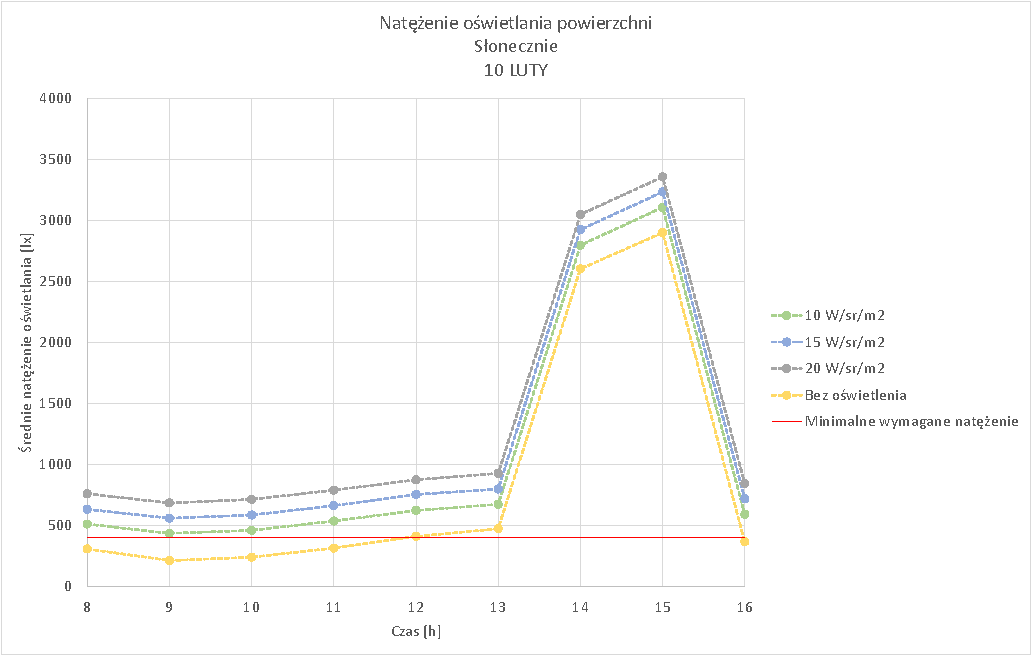
\includegraphics[scale=0.8]{Wykresy/oswietlenie_2_slonecznie.pdf}
		\caption{Natężenie oświetlania powierzchni biurka w sali lekcyjnej w słoneczny dzień przy włączonym oświetleniu dla konfiguracji opraw oświetleniowych nr 2 i różnej wartości radiancji}
		\label{oswietlenie_2_slonecznie}
	\end{figure}
	
	\begin{figure}[!ht]
		\centering
		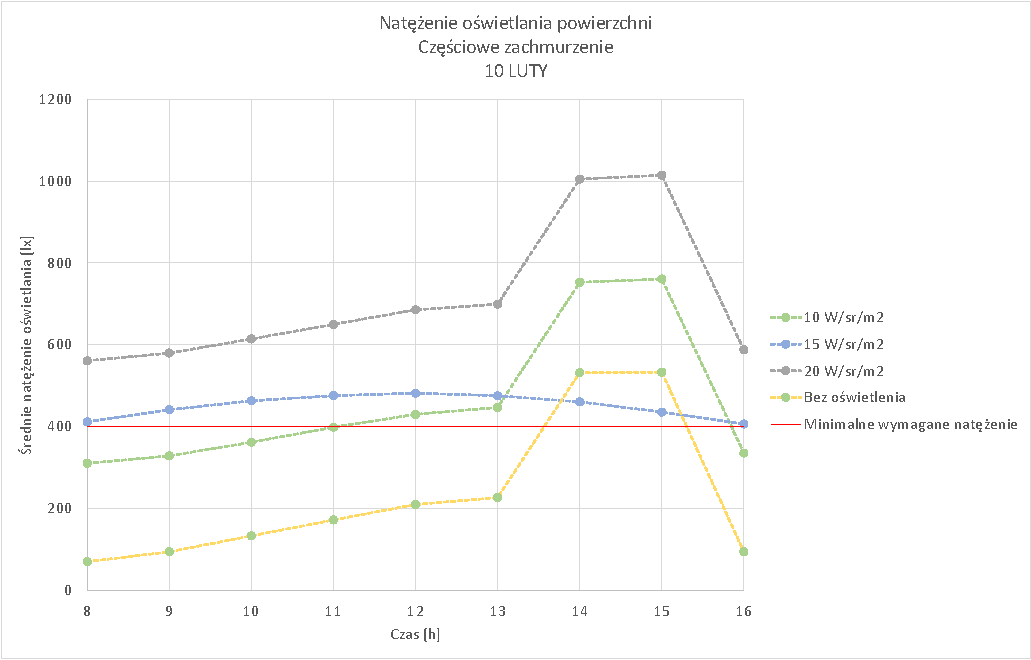
\includegraphics[scale=0.8]{Wykresy/oswietlenie_2_czesciowe_zachmurzenie.pdf}
		\caption{Natężenie oświetlania powierzchni biurka w sali lekcyjnej przy częściowym zachmurzeniu  oraz włączonym oświetleniu dla konfiguracji opraw oświetleniowych nr 2 i różnej wartości radiancji}
		\label{oswietlenie_2_czesciowe_zachmurzenie}
	\end{figure}
	
	\begin{figure}[!ht]
		\centering
		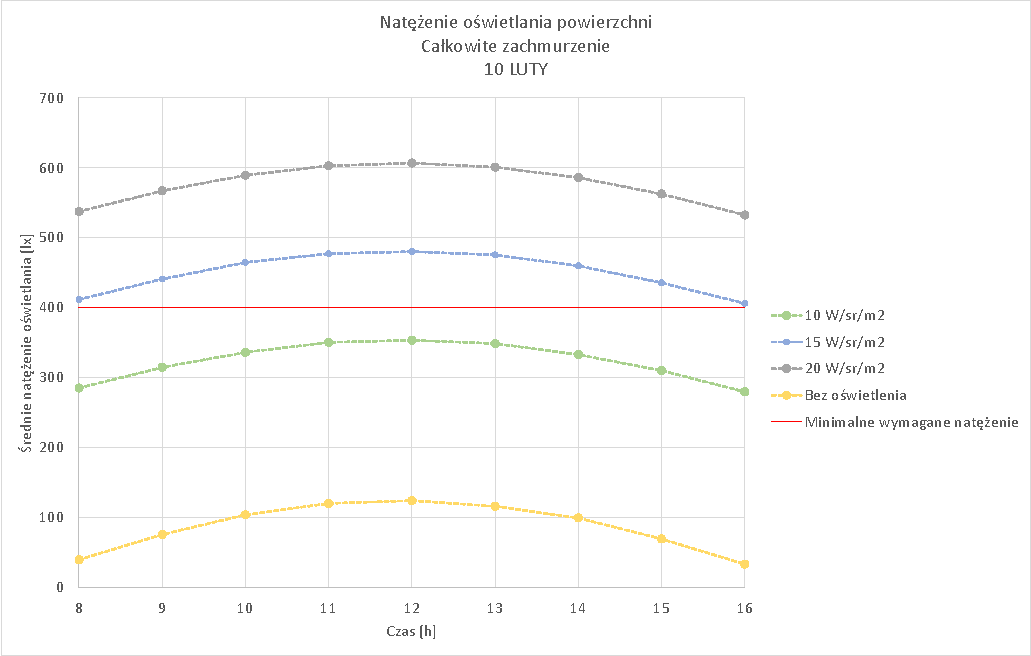
\includegraphics[scale=0.8]{Wykresy/oswietlenie_2_calkowite_zachmurzenie.pdf}
		\caption{Natężenie oświetlania powierzchni biurka w sali lekcyjnej przy całkowitym zachmurzeniu  oraz włączonym oświetleniu dla konfiguracji opraw oświetleniowych nr 2 i różnej wartości radiancji}
		\label{oswietlenie_2_calkowite_zachmurzenie}
	\end{figure}

	\clearpage
	\subsection{Zestawienie wybranych wyników}
	\label{subsec:zestawienie_wybranych_wynikow}
	
	\begin{figure}[!ht]
		\centering
		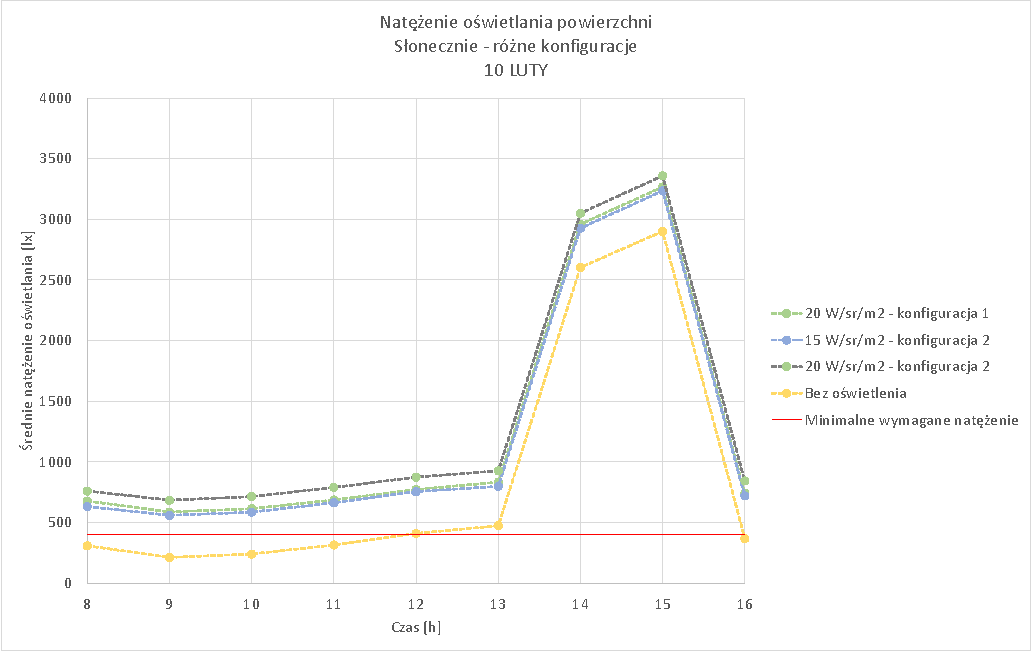
\includegraphics[scale=0.8]{Wykresy/oswietlenie_slonecznie_rozne_konfiguracje.pdf}
		\caption{Natężenie oświetlania powierzchni biurka w sali lekcyjnej w słoneczny dzień dla wybranych konfiguracji opraw oświetleniowych i wartości radiancji}
		\label{oswietlenie_slonecznie_rozne_konfiguracje}
	\end{figure}

	\begin{figure}[!ht]
		\centering
		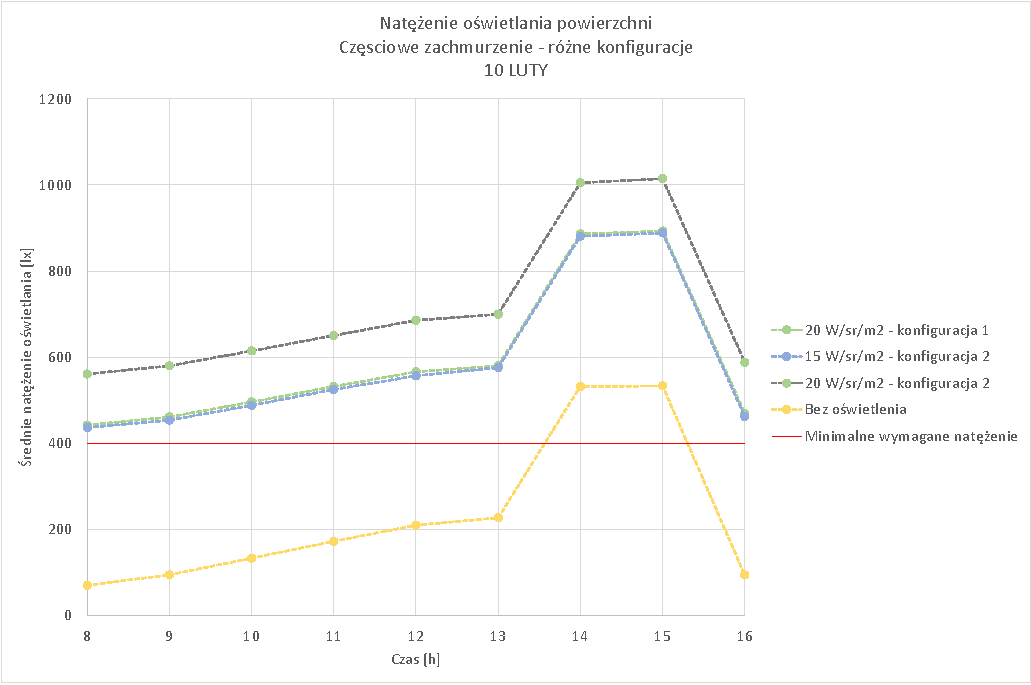
\includegraphics[scale=0.8]{Wykresy/oswietlenie_czesciowe_zachmurzenie_rozne_konfiguracje.pdf}
		\caption{Natężenie oświetlania powierzchni biurka w sali lekcyjnej przy częściowym zachmurzeniu  oraz włączonym oświetleniu dla wybranych konfiguracji opraw oświetleniowych i różnej wartości radiancji}
		\label{oswietlenie_czesciowe_zachmurzenie_rozne_konfiguracje}
	\end{figure}

	\begin{figure}[!ht]
		\centering
		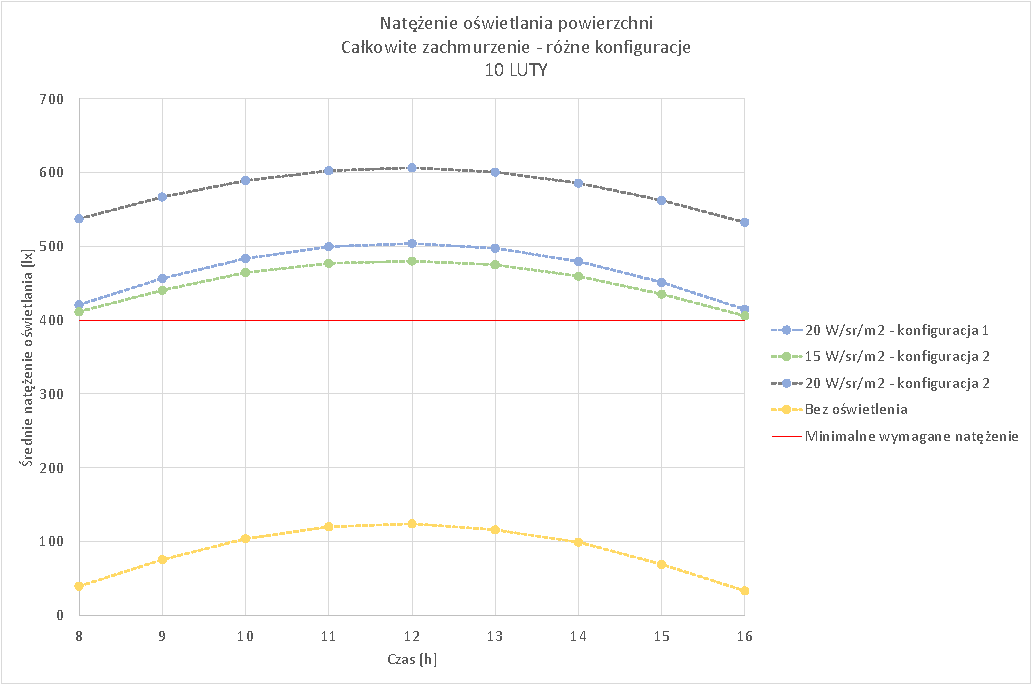
\includegraphics[scale=0.8]{Wykresy/oswietlenie_calkowite_zachmurzenie_rozne_konfiguracje.pdf}
		\caption{Natężenie oświetlania powierzchni biurka w sali lekcyjnej przy całkowitym zachmurzeniu  oraz włączonym oświetleniu dla wybranych konfiguracji opraw oświetleniowych i różnej wartości radiancji}
		\label{oswietlenie_calkowite_zachmurzenie_rozne_konfiguracje}
	\end{figure}

	\begin{figure}[!ht]
		\centering
		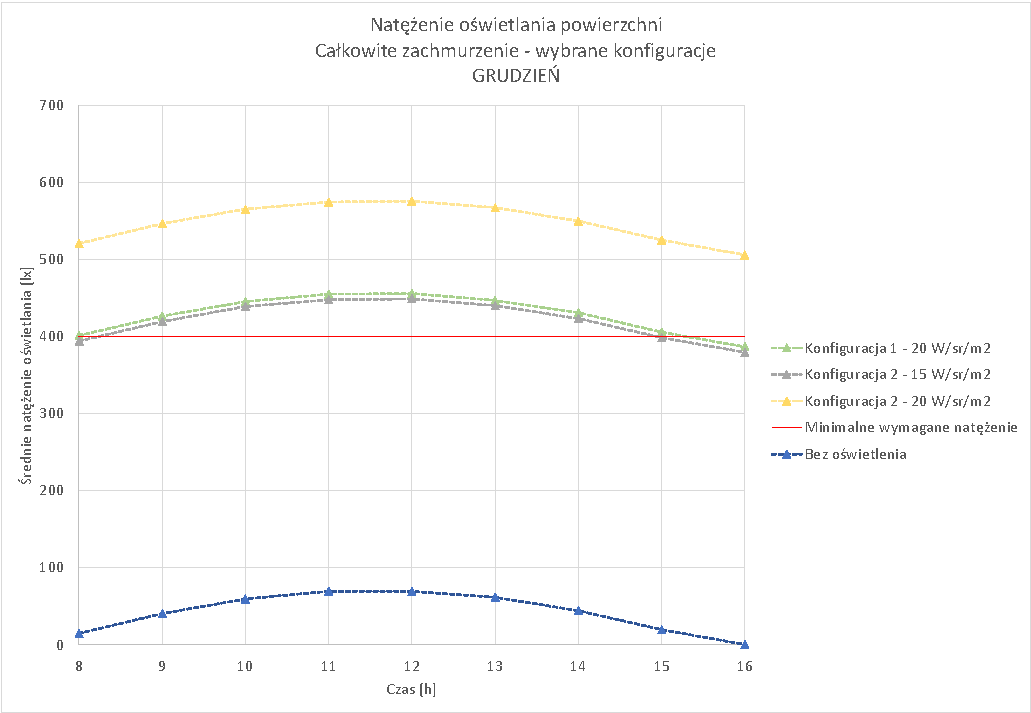
\includegraphics[scale=0.8]{Wykresy/grudzien_oswietlenie_calkowite_zachmurzenie_rozne_konfiguracje.pdf}
		\caption{Natężenie oświetlania powierzchni biurka w sali lekcyjnej przy całkowitym zachmurzeniu  w grudniu oraz włączonym oświetleniu dla wybranych konfiguracji opraw oświetleniowych i różnej wartości radiancji}
		\label{grudzien_oswietlenie_calkowite_zachmurzenie_rozne_konfiguracje}
	\end{figure}	


	\begin{figure}[!ht]
		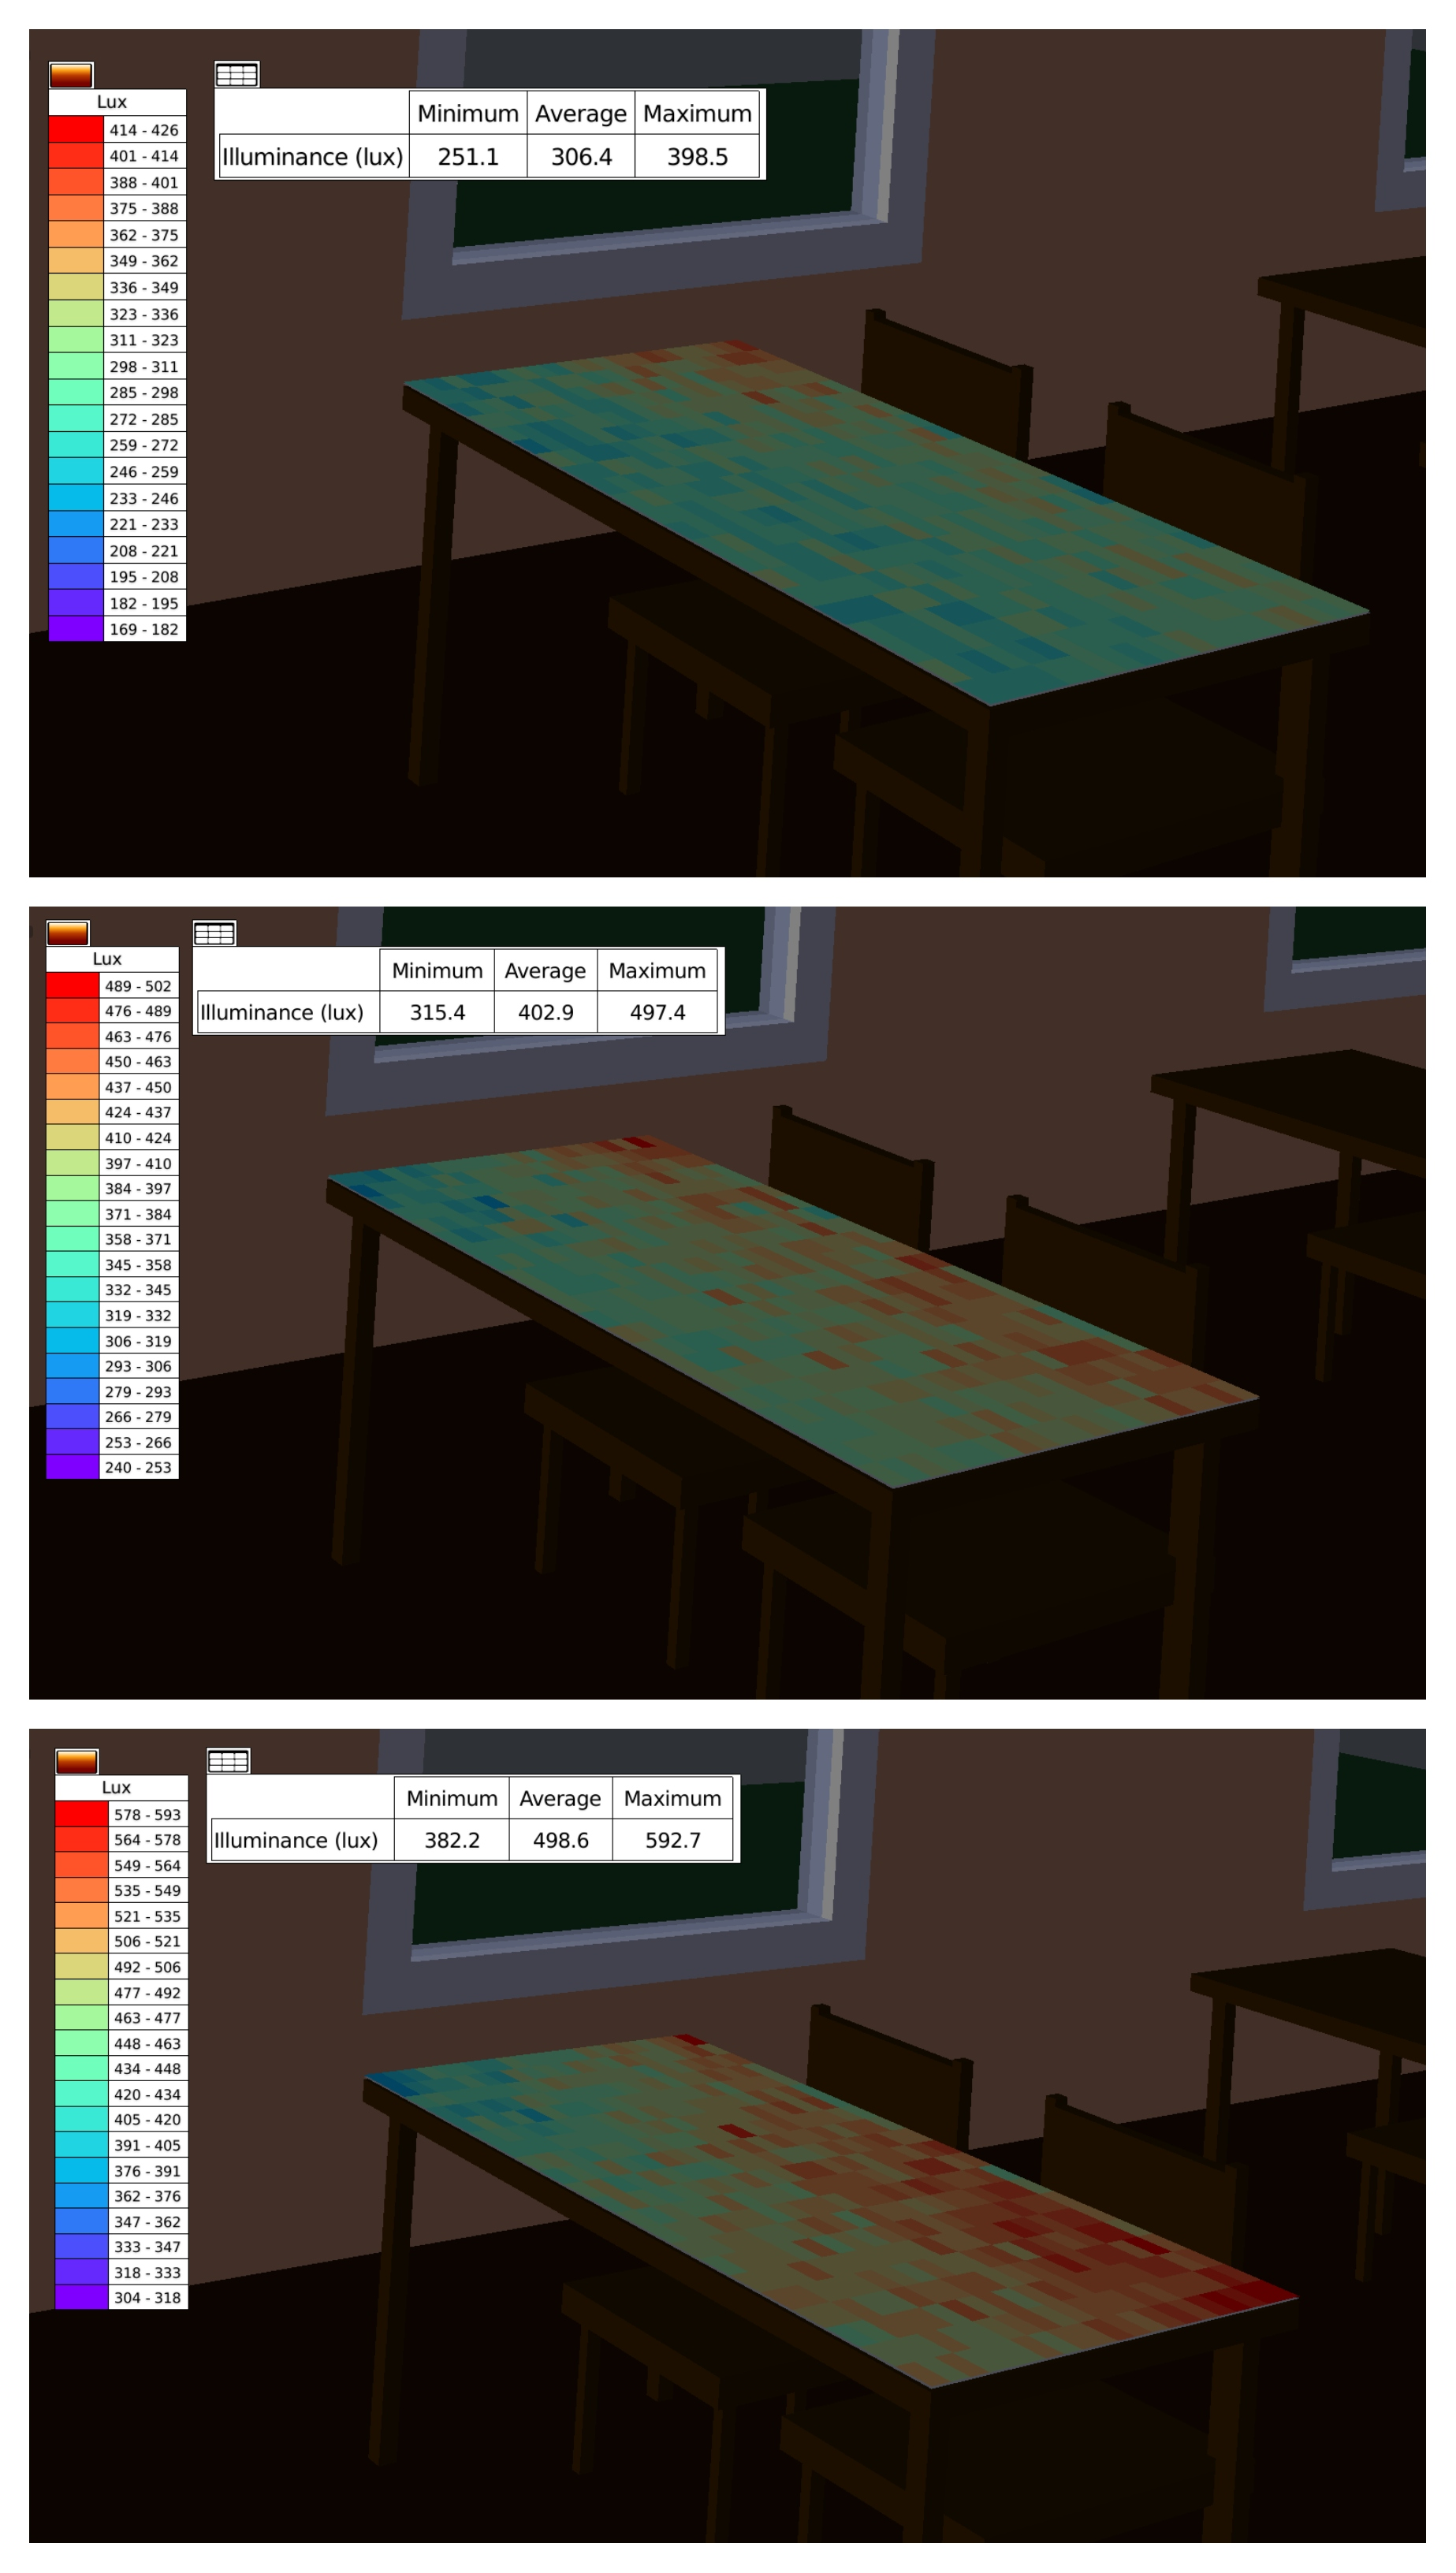
\includegraphics[scale=0.8]{wplyw_natezenia}
		\centering
		\caption{Wpływ zmiany natężenia lamp przy całkowitym zachmurzeniu dla miesiąca luty - godzina 13:00}
		\label{fig:wplyw_natezenia_symulacja}
	\end{figure}

	\begin{figure}[!th]
		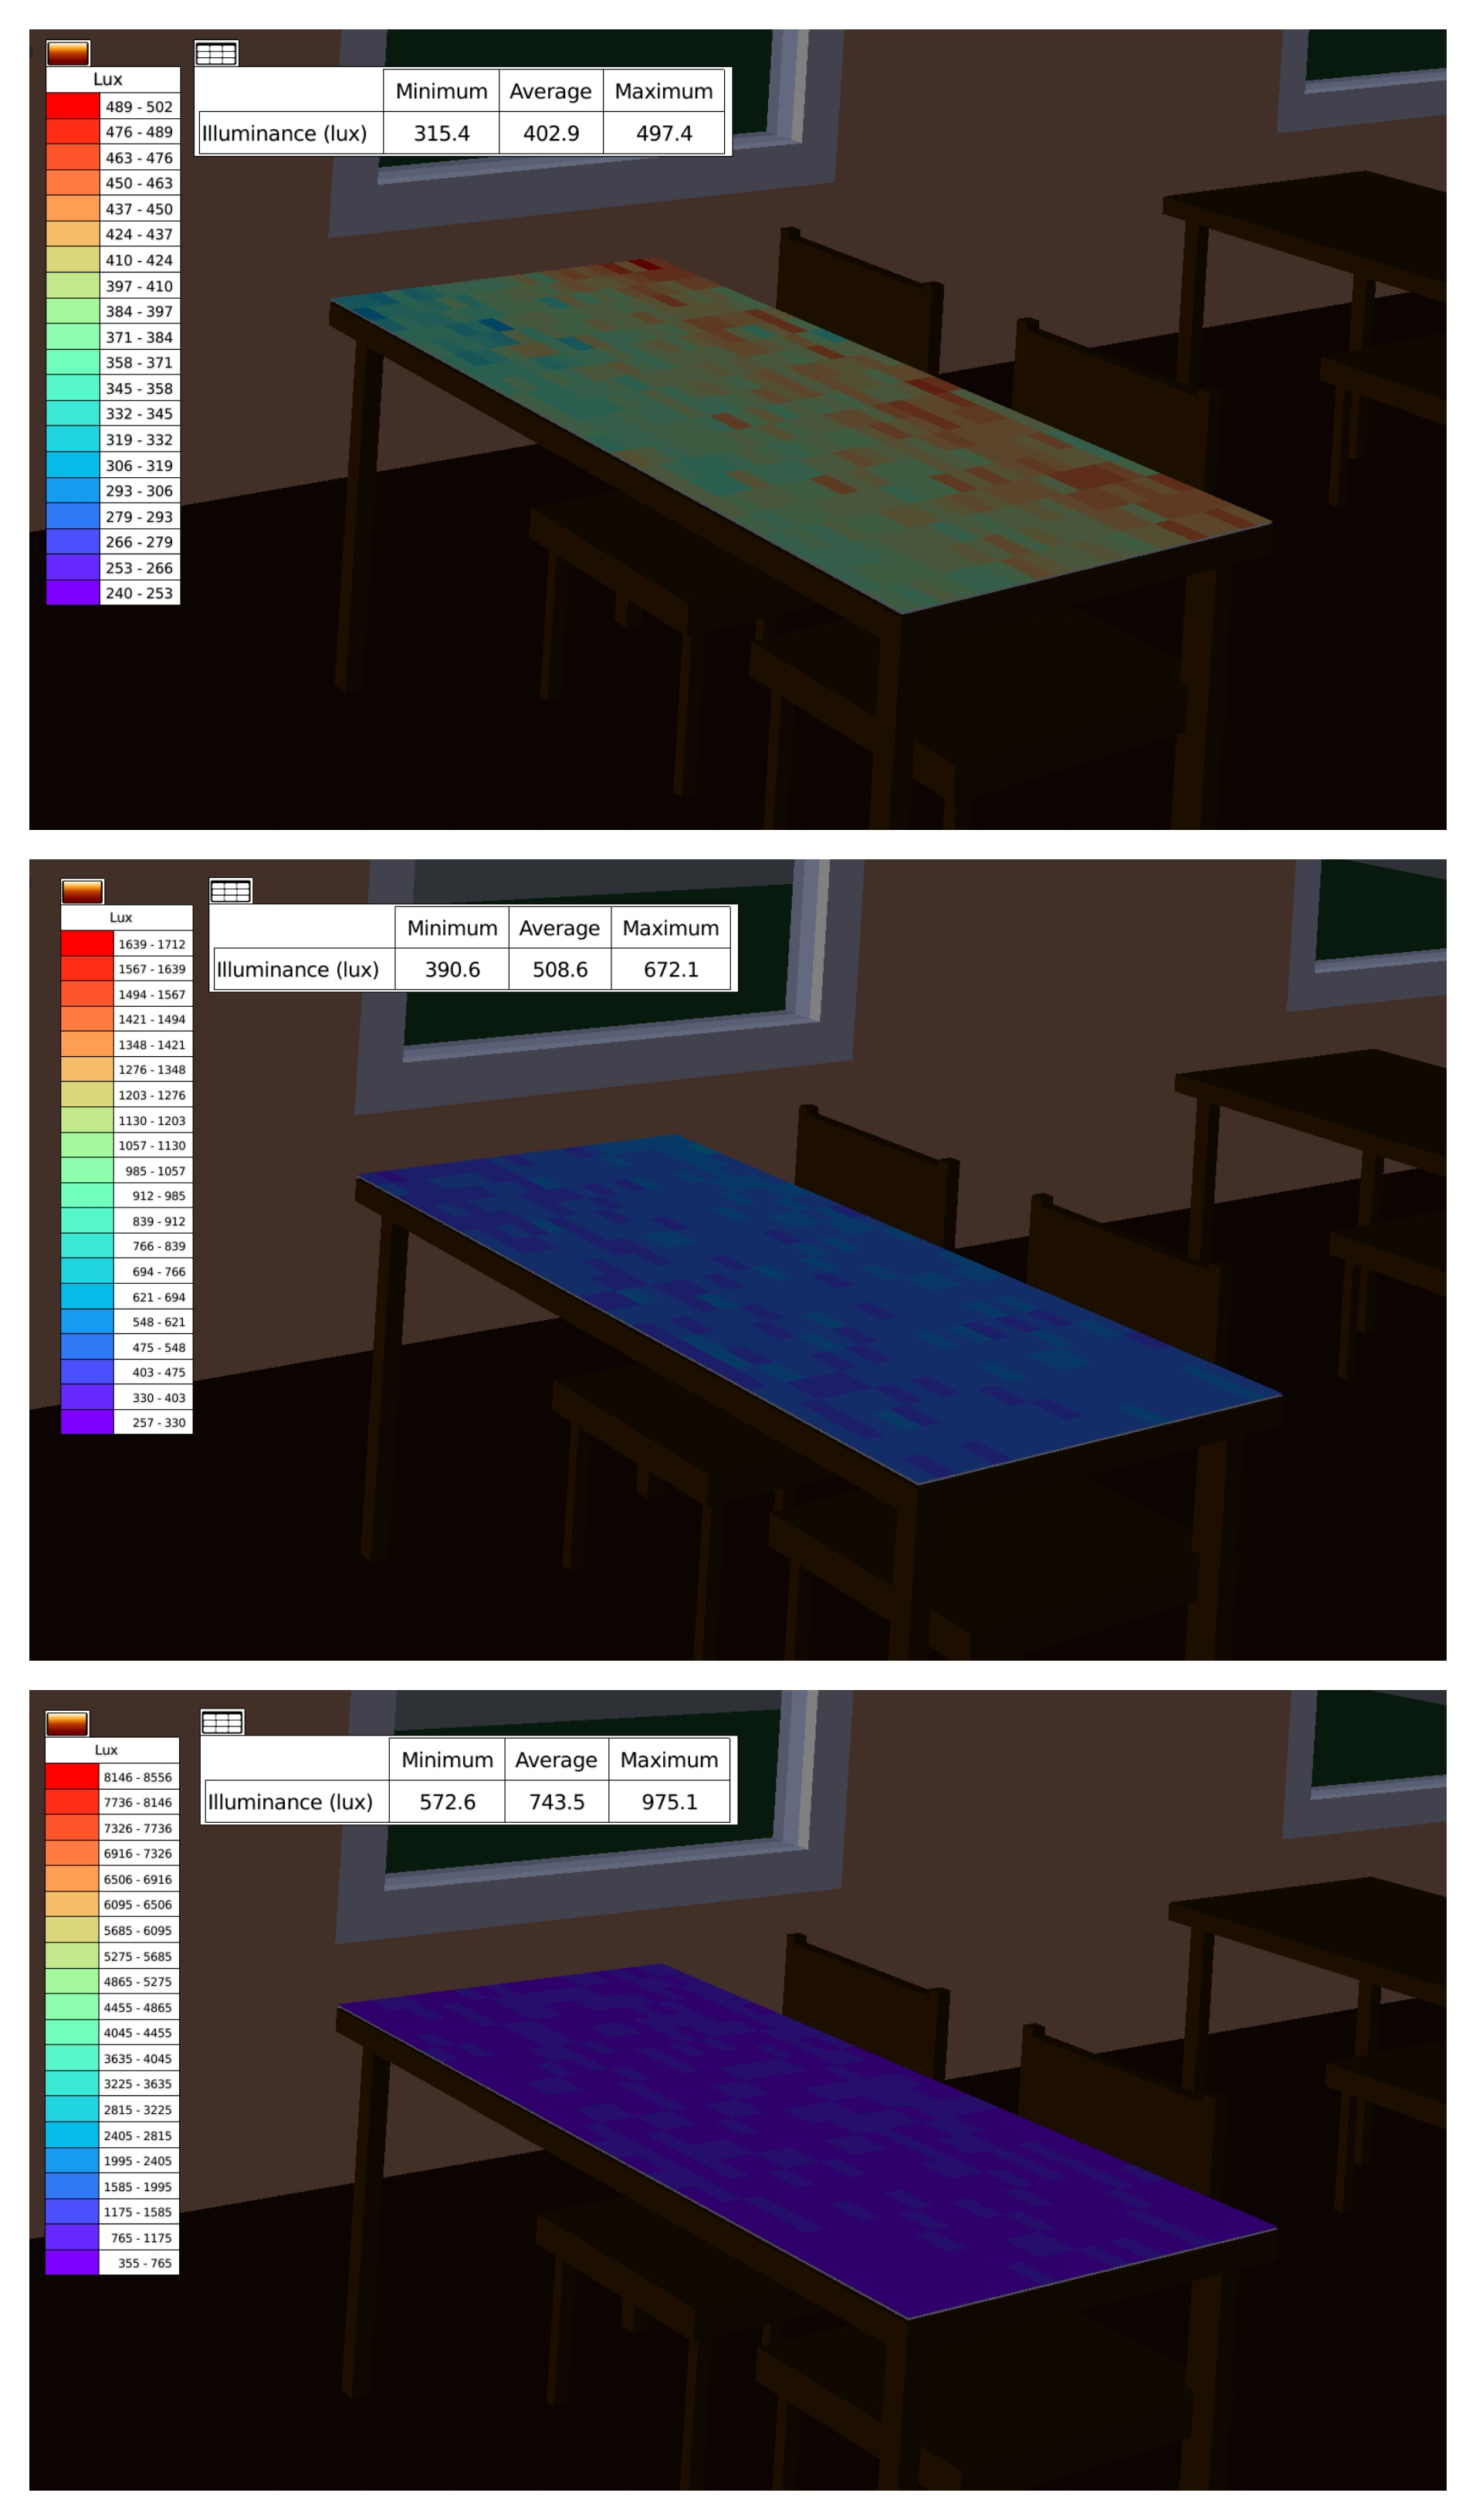
\includegraphics[scale=0.8]{wplyw_warunkow_pogodowych}
		\centering
		\caption{Wpływ zmiany warunków pogodowych przy stałym natężeniu dla miesiąca luty - godzina 13:00}
		\label{fig:wplyw_warunkow_pogodowych_symulacja}
	\end{figure}
	\clearpage	
	
	\section{Podsumowanie}
	\label{sec:podsumowanie}	

	\subsection{Dla wybranego miesiąca - luty}
	\label{subsec:podsumowanie_wybranego_miesiaca_luty}

	\begin{table}[!ht]
		\begin{tabular}{|c|c|c|c|c|c|c|c|c|c|}
			\hline
			\multicolumn{10}{|c|}{\cellcolor[HTML]{C8DFC8}Bez oświetlenia} \\ \hline
			\multicolumn{10}{|c|}{\cellcolor[HTML]{EDD9A0}Słonecznie} \\ \hline
	
			Godzina & \cellcolor[HTML]{FFFFFF}8 & \cellcolor[HTML]{FFFFFF}9 & \cellcolor[HTML]{FFFFFF}10 & \cellcolor[HTML]{FFFFFF}11 & \cellcolor[HTML]{FFFFFF}12 & \cellcolor[HTML]{FFFFFF}13 & \cellcolor[HTML]{FFFFFF}14 & \cellcolor[HTML]{FFFFFF}15 & \cellcolor[HTML]{FFFFFF}16 \\ \hline
			Śr. wartość natężenia oświetlenia {[}lux{]} & \cellcolor[HTML]{FFCCC9}307 & \cellcolor[HTML]{FFCCC9}211 & \cellcolor[HTML]{FFCCC9}240 & \cellcolor[HTML]{F6E9C3}314 & \cellcolor[HTML]{F6E9C3}409 & \cellcolor[HTML]{F6E9C3}473 & \cellcolor[HTML]{F6E9C3}2604 & \cellcolor[HTML]{F6E9C3}2901 & 							\cellcolor[HTML]{FFCCC9}367 \\ \hline
	
			\multicolumn{10}{|c|}{\cellcolor[HTML]{B2BFE5}Częściowe zachmurzenie} \\ \hline
			Godzina & \cellcolor[HTML]{FFFFFF}8 & \cellcolor[HTML]{FFFFFF}9 & \cellcolor[HTML]{FFFFFF}10 & \cellcolor[HTML]{FFFFFF}11 & \cellcolor[HTML]{FFFFFF}12 & \cellcolor[HTML]{FFFFFF}13 & \cellcolor[HTML]{FFFFFF}14 & \cellcolor[HTML]{FFFFFF}15 & \cellcolor[HTML]{FFFFFF}16 \\ \hline
			Śr. wartość natężenia oświetlenia {[}lux{]} & \cellcolor[HTML]{FFCCC9}{\color[HTML]{000000} 69} & \cellcolor[HTML]{FFCCC9}{\color[HTML]{000000} 94} & \cellcolor[HTML]{FFCCC9}{\color[HTML]{000000} 132} & \cellcolor[HTML]{FFCCC9}{\color[HTML]{000000} 171} & \cellcolor[HTML]{FFCCC9}{\color[HTML]						{000000} 209} & \cellcolor[HTML]{FFCCC9}{\color[HTML]{000000} 226} & \cellcolor[HTML]{C7D1EE}{\color[HTML]{000000} 531} & \cellcolor[HTML]{C7D1EE}{\color[HTML]{000000} 533} & \cellcolor[HTML]{FFCCC9}{\color[HTML]{000000} 94} \\ \hline
	
			\multicolumn{10}{|c|}{\cellcolor[HTML]{C3C3C3}Całkowite zachmurzenie} \\ \hline
			Godzina & 8 & 9 & 10 & 11 & 12 & 13 & 14 & 15 & 16 \\ \hline
			Śr. wartość natężenia oświetlenia {[}lux{]} & \cellcolor[HTML]{FFCCC9}{\color[HTML]{000000} 39} & \cellcolor[HTML]{FFCCC9}{\color[HTML]{000000} 75} & \cellcolor[HTML]{FFCCC9}{\color[HTML]{000000} 104} & \cellcolor[HTML]{FFCCC9}{\color[HTML]{000000} 120} & \cellcolor[HTML]{FFCCC9}{\color[HTML]						{000000} 124} & \cellcolor[HTML]{FFCCC9}{\color[HTML]{000000} 116} & \cellcolor[HTML]{FFCCC9}{\color[HTML]{000000} 99}  & \cellcolor[HTML]{FFCCC9}{\color[HTML]{000000} 69}  & \cellcolor[HTML]{FFCCC9}{\color[HTML]{000000} 33} \\ \hline
		\end{tabular}
		\caption{\label{tab:zmiany_natezenia_luty_brak_oswietlenia}Natężenie oświetlenia powierzchni biurka dla  miesiąca luty bez sztucznego oświetlenia}
	\end{table}

	W przypadku braku sztucznego oświetlenia, niezależnie od panujących warunków naturalnych, światło słoneczne nie jest wystarczające by zapewnić dobre oświetlenie spełniające wymagane normy 400 lx.

	\begin{table}[!ht]
		\begin{tabular}{|c|c|c|c|c|c|c|c|c|c|}
			\hline
			
			\multicolumn{10}{|c|}{\cellcolor[HTML]{C8DFC8}Konfiguracja opraw oświetleniowych 1} \\ \hline
			
			\multicolumn{10}{|c|}{\cellcolor[HTML]{EDD9A0}Słonecznie} \\ \hline
			Godzina & \cellcolor[HTML]{FFFFFF}8 & \cellcolor[HTML]{FFFFFF}9 & \cellcolor[HTML]{FFFFFF}10 & \cellcolor[HTML]{FFFFFF}11 & \cellcolor[HTML]{FFFFFF}12 & \cellcolor[HTML]{FFFFFF}13 & \cellcolor[HTML]{FFFFFF}14 & \cellcolor[HTML]{FFFFFF}15 & \cellcolor[HTML]{FFFFFF}16 \\ \hline
			
			\multicolumn{10}{|c|}{10 W/sr/$m^{2}$} \\ \hline
			Śr. wartość natężenie oświetlenia {[}lux{]} & \cellcolor[HTML]{F6E9C3}486 & \cellcolor[HTML]{FFCCC9}{\color[HTML]{000000} 398} & \cellcolor[HTML]{F6E9C3}422 & \cellcolor[HTML]{F6E9C3}496 & \cellcolor[HTML]{F6E9C3}583 & \cellcolor[HTML]{F6E9C3}646 & \cellcolor[HTML]{F6E9C3}2769 & \cellcolor[HTML]						{F6E9C3}3078 & \cellcolor[HTML]{F6E9C3}554 \\ \hline
			
			\multicolumn{10}{|c|}{15 W/sr/$m^{2}$} \\ \hline
			
			\multicolumn{1}{|l|}{Śr. wartość natężenia oświetlenia {[}lux{]}} & \cellcolor[HTML]{F6E9C3}548 & \cellcolor[HTML]{F6E9C3}475 & \cellcolor[HTML]{F6E9C3}499 & \cellcolor[HTML]{F6E9C3}577 & \cellcolor[HTML]{F6E9C3}669 & \cellcolor[HTML]{F6E9C3}716 & \cellcolor[HTML]{F6E9C3}2846 & \cellcolor[HTML]{F6E9C3}					3158 & \cellcolor[HTML]{F6E9C3}629 \\ \hline
			
			\multicolumn{10}{|c|}{20 W/sr/$m^{2}$} \\ \hline
			
			\multicolumn{1}{|l|}{Śr. wartość natężenia oświetlenia {[}lux{]}} & \cellcolor[HTML]{F6E9C3}677 & \cellcolor[HTML]{F6E9C3}587 & \cellcolor[HTML]{F6E9C3}614 & \cellcolor[HTML]{F6E9C3}686 & \cellcolor[HTML]{F6E9C3}771 & \cellcolor[HTML]{F6E9C3}832 & \cellcolor[HTML]{F6E9C3}2961 & \cellcolor[HTML]{F6E9C3}					3267 & \cellcolor[HTML]{F6E9C3}741 \\ \hline
			
			\multicolumn{10}{|c|}{\cellcolor[HTML]{B2BFE5}Częściowe zachmurzenie} \\ \hline
			Godzina & \cellcolor[HTML]{FFFFFF}8 & \cellcolor[HTML]{FFFFFF}9 & \cellcolor[HTML]{FFFFFF}10 & \cellcolor[HTML]{FFFFFF}11 & \cellcolor[HTML]{FFFFFF}12 & \cellcolor[HTML]{FFFFFF}13 & \cellcolor[HTML]{FFFFFF}14 & \cellcolor[HTML]{FFFFFF}15 & \cellcolor[HTML]{FFFFFF}16 \\ \hline
			
			\multicolumn{10}{|c|}{10 W/sr/$m^{2}$} \\ \hline
			Śr. wartość natężenia oświetlenia {[}lux{]} & \cellcolor[HTML]{FFCCC9}{\color[HTML]{330001} 259} & \cellcolor[HTML]{FFCCC9}{\color[HTML]{330001} 284} & \cellcolor[HTML]{FFCCC9}{\color[HTML]{330001} 320} & \cellcolor[HTML]{FFCCC9}{\color[HTML]{330001} 360} & \cellcolor[HTML]{FFCCC9}{\color[HTML]					{330001} 394} & \cellcolor[HTML]{CDD6F1}{\color[HTML]{330001} 413} & \cellcolor[HTML]{CDD6F1}{\color[HTML]{330001} 718} & \cellcolor[HTML]{CDD6F1}{\color[HTML]{330001} 717} & \cellcolor[HTML]{FFCCC9}{\color[HTML]{330001} 284} \\ \hline
			
			\multicolumn{10}{|c|}{15 W/sr/$m^{2}$} \\ \hline
			Śr. wartość natężenia oświetlenia {[}lux{]} & \cellcolor[HTML]{FFCCC9}{\color[HTML]{000000} 346} & \cellcolor[HTML]{FFCCC9}{\color[HTML]{000000} 365} & \cellcolor[HTML]{FFCCC9}{\color[HTML]{000000} 399} & \cellcolor[HTML]{CDD6F1}{\color[HTML]{000000} 435} & \cellcolor[HTML]{CDD6F1}{\color[HTML]					{000000} 470} & \cellcolor[HTML]{CDD6F1}{\color[HTML]{000000} 484} & \cellcolor[HTML]{CDD6F1}{\color[HTML]{000000} 791} & \cellcolor[HTML]{CDD6F1}{\color[HTML]{000000} 798} & \cellcolor[HTML]{FFCCC9}{\color[HTML]{000000} 373} \\ \hline
			
			\multicolumn{10}{|c|}{20 W/sr/$m^{2}$} \\ \hline
			Śr. wartość natężenia oświetlenia {[}lux{]} & \cellcolor[HTML]{CDD6F1}442 & \cellcolor[HTML]{CDD6F1}461 & \cellcolor[HTML]{CDD6F1}495 & \cellcolor[HTML]{CDD6F1}531 & \cellcolor[HTML]{CDD6F1}566 & \cellcolor[HTML]{CDD6F1}580 & \cellcolor[HTML]{CDD6F1}886 & \cellcolor[HTML]{CDD6F1}893 & 							\cellcolor[HTML]{CDD6F1}469 \\ \hline
			
			\multicolumn{10}{|c|}{\cellcolor[HTML]{C3C3C3}Całkowite zachmurzenie} \\ \hline
			Godzina & 8 & 9 & 10 & 11 & 12 & 13 & 14 & 15 & 16 \\ \hline
			
			\multicolumn{10}{|c|}{10 W/sr/$m^{2}$} \\ \hline
			Śr. wartość natężenia oświetlenia {[}lux{]}& \cellcolor[HTML]{FFCCC9}{\color[HTML]{000000} 230} & \cellcolor[HTML]{FFCCC9}{\color[HTML]{000000} 266} & \cellcolor[HTML]{FFCCC9}{\color[HTML]{000000} 293} & \cellcolor[HTML]{FFCCC9}{\color[HTML]{000000} 309} & \cellcolor[HTML]{FFCCC9}{\color[HTML]					{000000} 314} & \cellcolor[HTML]{FFCCC9}{\color[HTML]{000000} 307} & \cellcolor[HTML]{FFCCC9}{\color[HTML]{000000} 289} & \cellcolor[HTML]{FFCCC9}{\color[HTML]{000000} 260} & \cellcolor[HTML]{FFCCC9}{\color[HTML]{000000} 224} \\ \hline
			
			\multicolumn{10}{|c|}{15 W/sr/$m^{2}$} \\ \hline
			Śr. wartość natężenia oświetlenia {[}lux{]} & \cellcolor[HTML]{FFCCC9}{\color[HTML]{000000} 322} & \cellcolor[HTML]{FFCCC9}{\color[HTML]{000000} 351} & \cellcolor[HTML]{FFCCC9}{\color[HTML]{000000} 373} & \cellcolor[HTML]{FFCCC9}{\color[HTML]{000000} 387} & \cellcolor[HTML]{FFCCC9}{\color[HTML]					{000000} 392} & \cellcolor[HTML]{FFCCC9}{\color[HTML]{000000} 385} & \cellcolor[HTML]{FFCCC9}{\color[HTML]{000000} 370} & \cellcolor[HTML]{FFCCC9}{\color[HTML]{000000} 347} & \cellcolor[HTML]{FFCCC9}{\color[HTML]{000000} 316} \\ \hline
			
			\multicolumn{10}{|c|}{20 W/sr/$m^{2}$} \\ \hline
			Śr. wartość natężenia oświetlenia {[}lux{]} & \cellcolor[HTML]{D9D9D9}{\color[HTML]{000000} 421} & \cellcolor[HTML]{D9D9D9}{\color[HTML]{000000} 457} & \cellcolor[HTML]{D9D9D9}{\color[HTML]{000000} 484} & \cellcolor[HTML]{D9D9D9}{\color[HTML]{000000} 500} & \cellcolor[HTML]{D9D9D9}{\color[HTML]					{000000} 504} & \cellcolor[HTML]{D9D9D9}{\color[HTML]{000000} 497} & \cellcolor[HTML]{D9D9D9}{\color[HTML]{000000} 480} & \cellcolor[HTML]{D9D9D9}{\color[HTML]{000000} 451} & \cellcolor[HTML]{D9D9D9}{\color[HTML]{000000} 415} \\ \hline

		\end{tabular}
		\caption{\label{tab:zmiany_natezenia_luty_oswietlenie_1}Natężenie oświetlenia powierzchni biurka dla  miesiąca luty dla konfiguracji opraw oświetleniowych~1}

	\end{table}
	\clearpage

	Dla pierwszej konfiguracji opraw oświetleniowych w sytuacji, gdy warunki są najbardziej korzystne lampa 15 W/sr/$m^{2}$ wydaje się być wystarczająca jednak, dla nieco pogorszonych  warunków pogodowych, nie spełnia ona norm. Należałoby zatem wybrać oświetlenie wynoszące 20 W/sr/$m^{2}$ dla takiego ustawienia.


	\begin{table}[!ht]
		\begin{tabular}{|c|c|c|c|c|c|c|c|c|c|}

			\hline
			\multicolumn{10}{|c|}{\cellcolor[HTML]{C8DFC8}Konfiguracja opraw oświetleniowych 2} \\ \hline
		
			\multicolumn{10}{|c|}{\cellcolor[HTML]{EDD9A0}Słonecznie} \\ \hline
			Godzina & \cellcolor[HTML]{FFFFFF}8 & \cellcolor[HTML]{FFFFFF}9 & \cellcolor[HTML]{FFFFFF}10 & \cellcolor[HTML]{FFFFFF}11 & \cellcolor[HTML]{FFFFFF}12 & \cellcolor[HTML]{FFFFFF}13 & \cellcolor[HTML]{FFFFFF}14 & \cellcolor[HTML]{FFFFFF}15 & \cellcolor[HTML]{FFFFFF}16 \\ \hline
	
			\multicolumn{10}{|c|}{10 W/sr/$m^{2}$} \\ \hline
			Śr. wartość natężenia oświetlenia {[}lux{]} & \cellcolor[HTML]{F6E9C3}511 & \cellcolor[HTML]{F6E9C3}{\color[HTML]{000000} 435} & \cellcolor[HTML]{F6E9C3}460 & \cellcolor[HTML]{F6E9C3}536 & \cellcolor[HTML]{F6E9C3}623 & \cellcolor[HTML]{F6E9C3}673 & \cellcolor[HTML]{F6E9C3}2799 & \cellcolor[HTML]						{F6E9C3}3108 & \cellcolor[HTML]{F6E9C3}591 \\ \hline
	
			\multicolumn{10}{|c|}{15 W/sr/$m^{2}$} \\ \hline
			Śr. wartość natężenia oświetlenia {[}lux{]} & \cellcolor[HTML]{F6E9C3}631 & \cellcolor[HTML]{F6E9C3}559 & \cellcolor[HTML]{F6E9C3}585 & \cellcolor[HTML]{F6E9C3}663 & \cellcolor[HTML]{F6E9C3}754 & \cellcolor[HTML]{F6E9C3}798 & \cellcolor[HTML]{F6E9C3}2926 & \cellcolor[HTML]{F6E9C3}3235 & 							\cellcolor[HTML]{F6E9C3}719 \\ \hline
	
			\multicolumn{10}{|c|}{20 W/sr/$m^{2}$} \\ \hline
			Śr. wartość natężenia oświetlenia {[}lux{]} & \cellcolor[HTML]{F6E9C3}759 & \cellcolor[HTML]{F6E9C3}684 & \cellcolor[HTML]{F6E9C3}713 & \cellcolor[HTML]{F6E9C3}789 & \cellcolor[HTML]{F6E9C3}874 & \cellcolor[HTML]{F6E9C3}927 & \cellcolor[HTML]{F6E9C3}3051 & \cellcolor[HTML]{F6E9C3}3359 & 							\cellcolor[HTML]{F6E9C3}843 \\ \hline
	
			\multicolumn{10}{|c|}{\cellcolor[HTML]{B2BFE5}Częściowe zachmurzenie} \\ \hline
			Godzina & \cellcolor[HTML]{FFFFFF}8 & \cellcolor[HTML]{FFFFFF}9 & \cellcolor[HTML]{FFFFFF}10 & \cellcolor[HTML]{FFFFFF}11 & \cellcolor[HTML]{FFFFFF}12 & \cellcolor[HTML]{FFFFFF}13 & \cellcolor[HTML]{FFFFFF}14 & \cellcolor[HTML]{FFFFFF}15 & \cellcolor[HTML]{FFFFFF}16 \\ \hline
	
			\multicolumn{10}{|c|}{10 W/sr/$m^{2}$} \\ \hline
			Śr. wartość natężenia oświetlenia {[}lux{]} & \cellcolor[HTML]{FFCCC9}{\color[HTML]{000000} 310} & \cellcolor[HTML]{FFCCC9}{\color[HTML]{000000} 328} & \cellcolor[HTML]{FFCCC9}{\color[HTML]{000000} 362} & \cellcolor[HTML]{FFCCC9}{\color[HTML]{000000} 398} & \cellcolor[HTML]{D6DEF7}{\color[HTML]					{330001}430} & \cellcolor[HTML]{D6DEF7}{\color[HTML]{330001} 447} & \cellcolor[HTML]{D6DEF7}{\color[HTML]{330001} 753} & \cellcolor[HTML]{D6DEF7}{\color[HTML]{330001} 760} & \cellcolor[HTML]{FFCCC9}{\color[HTML]{000000} 335} \\ \hline
	
			\multicolumn{10}{|c|}{15 W/sr/$m^{2}$} \\ \hline
			Śr. wartość natężenia oświetlenia {[}lux{]} & \cellcolor[HTML]{D6DEF7}{\color[HTML]{000000} 436} & \cellcolor[HTML]{D6DEF7}{\color[HTML]{000000} 453} & \cellcolor[HTML]{D6DEF7}{\color[HTML]{000000} 488} & \cellcolor[HTML]{D6DEF7}{\color[HTML]{000000} 524} & \cellcolor[HTML]{D6DEF7}{\color[HTML]					{000000}556} & \cellcolor[HTML]{D6DEF7}{\color[HTML]{000000} 575} & \cellcolor[HTML]{D6DEF7}{\color[HTML]{000000} 881} & \cellcolor[HTML]{D6DEF7}{\color[HTML]{000000} 888} & \cellcolor[HTML]{D6DEF7}{\color[HTML]{000000} 462} \\ \hline
	
			\multicolumn{10}{|c|}{20 W/sr/$m^{2}$} \\ \hline
			Śr. wartość natężenia oświetlenia {[}lux{]} & \cellcolor[HTML]{D6DEF7}561 & \cellcolor[HTML]{D6DEF7}579 & \cellcolor[HTML]{D6DEF7}614 & \cellcolor[HTML]{D6DEF7}650 & \cellcolor[HTML]{D6DEF7}685 & \cellcolor[HTML]{D6DEF7}699 & \cellcolor[HTML]{D6DEF7}1005 & \cellcolor[HTML]{D6DEF7}1015 & 							\cellcolor[HTML]{D6DEF7}588 \\ \hline
	
			\multicolumn{10}{|c|}{\cellcolor[HTML]{C3C3C3}Całkowite zachmurzenie} \\ \hline
			Godzina & 8 & 9 & 10 & 11 & 12 & 13 & 14 & 15 & 16 \\ \hline
	
			\multicolumn{10}{|c|}{10 W/sr/$m^{2}$} \\ \hline
			Śr. wartość natężenia oświetlenia {[}lux{]} & \cellcolor[HTML]{FFCCC9}{\color[HTML]{000000} 285} & \cellcolor[HTML]{FFCCC9}{\color[HTML]{000000} 315} & \cellcolor[HTML]{FFCCC9}{\color[HTML]{000000} 336} & \cellcolor[HTML]{FFCCC9}{\color[HTML]{000000} 350} & \cellcolor[HTML]{FFCCC9}{\color[HTML]					{000000}353} & \cellcolor[HTML]{FFCCC9}{\color[HTML]{000000} 348} & \cellcolor[HTML]{FFCCC9}{\color[HTML]{000000} 333} & \cellcolor[HTML]{FFCCC9}{\color[HTML]{000000} 310} & \cellcolor[HTML]{FFCCC9}{\color[HTML]{000000} 280} \\ \hline
	
			\multicolumn{10}{|c|}{15 W/sr/$m^{2}$} \\ \hline
			Śr. wartość natężenia oświetlenia {[}lux{]} & \cellcolor[HTML]{D9D9D9}{\color[HTML]{000000} 412} & \cellcolor[HTML]{D9D9D9}{\color[HTML]{000000} 441} & \cellcolor[HTML]{D9D9D9}{\color[HTML]{000000} 465} & \cellcolor[HTML]{D9D9D9}{\color[HTML]{000000} 477} & \cellcolor[HTML]{D9D9D9}{\color[HTML]					{000000}480} & \cellcolor[HTML]{D9D9D9}{\color[HTML]{000000} 475} & \cellcolor[HTML]{D9D9D9}{\color[HTML]{000000} 460} & \cellcolor[HTML]{D9D9D9}{\color[HTML]{000000} 435} & \cellcolor[HTML]{D9D9D9}{\color[HTML]{000000} 406} \\ \hline
	
			\multicolumn{10}{|c|}{20 W/sr/$m^{2}$} \\ \hline
			Śr. wartość natężenia oświetlenia {[}lux{]} & \cellcolor[HTML]{D9D9D9}{\color[HTML]{000000} 537} & \cellcolor[HTML]{D9D9D9}{\color[HTML]{000000} 567} & \cellcolor[HTML]{D9D9D9}{\color[HTML]{000000} 589} & \cellcolor[HTML]{D9D9D9}{\color[HTML]{000000} 603} & \cellcolor[HTML]{D9D9D9}{\color[HTML]					{000000}607} & \cellcolor[HTML]{D9D9D9}{\color[HTML]{000000} 601} & \cellcolor[HTML]{D9D9D9}{\color[HTML]{000000} 586} & \cellcolor[HTML]{D9D9D9}{\color[HTML]{000000} 563} & \cellcolor[HTML]{D9D9D9}{\color[HTML]{000000} 533} \\ \hline

		\end{tabular}
		\caption{\label{tab:zmiany_natezenia_luty_oswietlenie_2}Natężenie oświetlenia powierzchni biurka dla  miesiąca luty dla konfiguracji opraw oświetleniowych~2}

	\end{table}

	W ostatnim przypadku, gdzie została użyta druga konfiguracja opraw, wybranie lamp 20 W/sr/$m^{2}$  pozwoli nam na uzyskanie oświetlenia spełniającego normy lecz z przyczyn ekonomicznych korzystniej byłoby wybrać lampy o nieco słabszej mocy 15 W/sr/$m^{2}$, które równej dobrze mogą zapewnić tak samo dobre 				warunki do pracy.

	\subsection{Dla całego roku}
	\label{subsec:podsumowanie_calego_roku}
	Po przeprowadzeniu symualcji dla całego roku, gdzie nie zostało użyte żadne dodatkowe naświetlenie pomieszczenia poza naturalnym, możemy zaobserwować brak spełnienia norm dla każdego miesiąca.
	Doświadczenie zostało wykonane dla całkowitego zachmurzenia nieba kiedy to warunki pogodowe są najmniej korzystne.
	Dla cieplejszych dni oświetlenie osiąga co najwyżej 211 lx - co wciąż jest dwa razy mniejsze od wymaganych regulacji. W przypadku zaś chłodniejszych miesięcy wynosi blisko 0 lx.
	Niestosowanie żadnego dodatkowego źródła światła przez cały rok nie jest możliwe.
	
	\clearpage

	\begin{table}[!ht]
		\begin{center}
		\begin{tabular}{c|
			>{\columncolor[HTML]{FFFFFF}}c |
			>{\columncolor[HTML]{FFFFFF}}c |
			>{\columncolor[HTML]{FFFFFF}}c |
			>{\columncolor[HTML]{FFFFFF}}c |
			>{\columncolor[HTML]{FFFFFF}}c |
			>{\columncolor[HTML]{FFFFFF}}c |
			>{\columncolor[HTML]{FFFFFF}}c |
			>{\columncolor[HTML]{FFFFFF}}c |
			>{\columncolor[HTML]{FFFFFF}}c |}
			\cline{2-10} & \multicolumn{9}{c|}{\cellcolor[HTML]{C8DFC8}Godzina} \\ \cline{2-10} 
			                    & \cellcolor[HTML]{F6FEF6}8 & \cellcolor[HTML]{F6FEF6}9 & \cellcolor[HTML]{F6FEF6}10 & \cellcolor[HTML]{F6FEF6}11 & \cellcolor[HTML]{F6FEF6}12 & \cellcolor[HTML]{F6FEF6}13 & \cellcolor[HTML]{F6FEF6}14 & \cellcolor[HTML]{F6FEF6}15 & \cellcolor[HTML]{F6FEF6}16 \\ \cline{2-10} 
			                    & \multicolumn{9}{c|}{\cellcolor[HTML]{DAE8FC}Śr. wartość natężenia oświetlenia {[}lux{]}} \\ \hline
			\multicolumn{1}{|c|}{\cellcolor[HTML]{F8E2B4}Styczeń}     & 12  & 39   & 60   & 72   & 75   & 69   & 53   & 29   & 0       \\ \hline
			\multicolumn{1}{|c|}{\cellcolor[HTML]{F8E2B4}Luty}           & 32  & 61   & 84   & 98   & 102 & 96   & 81   & 58   & 27     \\ \hline
			\multicolumn{1}{|c|}{\cellcolor[HTML]{F8E2B4}Marzec}      & 68   & 98   & 121 & 132 & 136 & 131 & 115 & 90   & 58     \\ \hline
			\multicolumn{1}{|c|}{\cellcolor[HTML]{F8E2B4}Kwiecień}    & 110 & 139 & 159 & 171 & 171 & 168 & 151 & 124 & 91     \\ \hline
			\multicolumn{1}{|c|}{\cellcolor[HTML]{F8E2B4}Maj}            & 140 & 167 & 186 & 197 & 199 & 192 & 172 & 148 & 115   \\ \hline
			\multicolumn{1}{|c|}{\cellcolor[HTML]{F8E2B4}Czerwiec}   & 153 & 179 & 200 & 206 & 209 & 203 & 188 & 161 & 133   \\ \hline
			\multicolumn{1}{|c|}{\cellcolor[HTML]{F8E2B4}Lipiec}         & 147 & 174 & 196 & 206 & 211 & 205 & 188 & 165 & 133   \\ \hline
			\multicolumn{1}{|c|}{\cellcolor[HTML]{F8E2B4}Sierpień}     & 131 & 158 & 182 & 193 & 193 & 186 & 172 & 146 & 114   \\ \hline
			\multicolumn{1}{|c|}{\cellcolor[HTML]{F8E2B4}Wrzesień}   & 103 & 133 & 152 & 165 & 165 & 154 & 138 & 109 & 78     \\ \hline
			\multicolumn{1}{|c|}{\cellcolor[HTML]{F8E2B4}Październik}& 72   & 98   & 115 & 126 & 124 & 117 & 95   & 68   & 34     \\ \hline
			\multicolumn{1}{|c|}{\cellcolor[HTML]{F8E2B4}Listopad}    & 37   & 63   & 80   & 91   & 89   & 79   & 59   & 33   & 0        \\ \hline
			\multicolumn{1}{|c|}{\cellcolor[HTML]{F8E2B4}Grudzień}   & 15   & 41   & 59   & 69   & 69   & 62   & 44   & 20   & 0         \\ \hline
		\end{tabular}
		\caption{\label{tab:zmiany_natezenia_caly_rok}Natężenie oświetlenia powierzchni biurka dla całego roku bez sztucznego oświetlenia przy całkowitym zachmurzeniu}
		
		\end{center}
	\end{table}
	
	\section{Wnioski}
	\label{sec:wnioski}
	W powyższej pracy została przeprowadzona analiza oświetlenia sali lekcyjnej.
	Otrzymane wyniki zostały zobrazowane w formie graficznej w postaci wykresów.
	Przedstawione rezultaty pozwalają stwierdzić, że zarówno warunki pogodowe, rozkład lamp jak i ich natężenie mają istotny wpływ  na natężenie oświetlenia.	
	Przeprowadzone analizy pokazują jak istotną rolę pełni dobre oświetlenie w salach lekcyjnych.
	Jeśli jest tylko taka możliwość naturalne oświetlenie jest bardziej preferwane często jednak nie jest ono wystarczające.


	\section{Plan działania}
	\label{sec:plan_dzialania}
	\begin{enumerate}
		\item Wykonanie modelu sali lekcyjnej przy użyciu programu \emph{Blender} \checkmark
		\item Wykonanie modelu natynkowej oprawy oświetleniowej zgodnej ze specyfikacją, przy użyciu programu \emph{Blender} \checkmark
		\item Wstępny dobór konfiguracji opraw oświetleniowych \checkmark
		\item Nadanie parametrów/materiałów Vi-Suite obiektom biorącym udział w sumlacji \checkmark
		\item Sporządzenie schematu w Node Edytorze \checkmark
		\item Dobór parametrów przeprowadzanych symulacji \checkmark
		\item Przeprowadzenie symulacji przy użyciu pakietu \emph{VI-Suite} i zewnętrznej aplikacji \emph{Radiance} dla różnych konfiguracji wybranych parametrów. \checkmark
		\item Zbiorcze zestawienie i analiza otrzymanych wyników \checkmark
		\item Porównanie rezultatów z rzeczywistymi badaniami \checkmark
		\item Wnioski i podsumowanie \checkmark
		
	\end{enumerate}
	
	\section{Przegląd literatury}
	\label{sec:przeglad_literatury}
	\begin{thebibliography}{7}
		\bibitem{1}
		D.Heim, A. Kujawski, \textit{Rozkład natężenia oświetlenia dziennego dla prostych struktur zabudowy}
		\bibitem{2}
		K. Błażejczyk et al., \textit{Seasonal and regional differences in lighting conditions and their influence on melatonin secretion}, Quaestiones Geographicae, 33(3), 2014, 17--25
		\bibitem{3}
		M. Ayoub, \textit{A review on light transport algorithms and simulation tools to model daylighting inside buildings}, Solar Energy, 198, 2020, 623--642
		\bibitem{4}
		L. Bellia, F. Fragliasso, \textit{Automated daylight-linked control systems performance with illuminance sensors for side-lit offices in the Mediterranean area}, Automation in Construction, 100 , 2019, 145--162
		\bibitem{5}
		R. Southall, F. Biljecki, \textit{The VI-Suite: a set of environmental analysis tools with geospatial data applications}, Open Geospatial Data, Software and Standards, 2017, 2--23
		\bibitem{6}
		\textit{Recommended Light Levels (Illuminance) for Outdoor and Indoor Venues}
		\bibitem{7}
		V. Logar, Z. Kristl, I. Skrjanc, \textit{Using a fuzzy black-box model to estimate the indoor illuminance in buildings}, Energy and Buildings, 70, 2014, 343--351
		\bibitem{8}
		Jerzy Wójcik Architekt IARP, "Szkoły podstawowe,szkoły średnie. Technologia obiektów", 28.10.2014
		\bibitem{9}
		http://www.instalacjebudowlane.pl/9490-29-12421-oswietlenie-led-w-szkolach--normy-i-rozwiazania-praktyczne.html
		\bibitem{10}
		Dr Ryan Southall, School of Art, Design \& Media - University of Brighton, Simulations and Visualisations with the VI-Suite - For VI-Suite Version 0.4
		\bibitem{11}
		https://energyplus.net/weather
		\bibitem{12}
		https://pl.wikipedia.org/wiki/Natezenie\_oswietlenia
		\bibitem{13}
		http://cmf.p.lodz.pl/iowczarek/materialy/fotometria/natenie\_owietlenia
		\bibitem{14}
		https://bezel.com.pl/2018/08/01/wymagania-oswietleniowe/	
	\end{thebibliography}
	
\end{document}